\documentclass[12pt]{article}

\usepackage[margin=1in]{geometry}  % set the margins to 1in on all sides
\usepackage{graphicx}              % to include figures
\usepackage{amsmath, bm}               % great math stuff
\usepackage{amsfonts}              % for blackboard bold, etc
\usepackage{amsthm}                % better theorem environments
\usepackage{hyperref}
\usepackage{natbib}
\usepackage{pdfpages}
\usepackage{booktabs}
\usepackage{multirow}

\newcommand{\kron}{\raisebox{1pt}{\ensuremath{\:\otimes\:}}} 
\newcommand{\lgamma}{\text{lgamma}} 
\newcommand{\digamma}{\text{digamma}} 

\bibliographystyle{plainnat}

\begin{document}

\nocite{*}

\title{Calibrating the pollen-vegetation relationship}

\author{Andria Dawson, Christopher Paciorek, Jason McLachlan,\\ Simon Goring, John Williams, Stephen Jackson}

\maketitle

\section{Introduction}

Understanding forest ecosystems of the past can provide us with
valuable information about how ecosystems respond to biotic and
abiotic factors. In particular, mapping forests back through time
offers new information not only about the climate-forest relationship,
but also forest-atmosphere interactions. In order to quantify forest
ecosystem change through time, we need spatio-temporal data. There is
no forest data that extends back through the last several millenia,
but there is a wealth of paleo-data, including fossil pollen data,
that serves as a proxy for surrounding vegetation. To make use of this
data to estimate past forest composition relies on our ability to
quantify the pollen-vegetation relationship. 

The complex nature of the pollen-vegetation relationship has been a
persistent theme in the paleoecological literature.
XXX Describe some of the research here....

Here, we describe the pollen-vegetation relationship using a Bayesian
hierarchical modelling framework developed by
\citet{paciorek2009mapping}. Pollen counts from a network of ponds are
modelled as a function of gridded forest composition data, taking into
account pollen dispersal from vegetation that is both local and
non-local to each pond, differential pollen production, and process
uncertainty. Using a Bayesian hierarchical model allows us to borrow
information across space to estimate governing parameters at a
regional scale, as well as estimate the uncertainty associated with
these parameters.

Sampling to quantify pollen-vegetation relationships usually involves
collecting surface sediment samples to obtain pollen counts at the
time of sampling, as well as a survey of vegetation composition and
abundance of the surrounding forests. Inference can then be made about
processes that affect pollen production, dispersal, and deposition for
the time that corresponds with time of sampling. To make inference
about these processes for times prior to the time of sampling requires
the assumption that the pollen-vegetation relationship is
stationary. Widespread land-use changes make it unlikely that this
assumption holds true for any length of time - at the very least, we
know that dramatic changes on the landscape affect pollen release and
transport by altering microclimatic factors including wind
dynamics. To circumvent these issues, we calibrate the pollen-vegetation
relationship using forest composition and sediment pollen data that
pre-dates European settlement, thereby avoiding the effects of
settlement, agriculture, and industrialization. 

There are few data sets that describe forest composition prior to the
twentieth century, which limits our understanding of pollen-vegetation
processes at past times. However, US Public Land Survey (PLS) records
collected by surveyors prior to European settlement provide us with an
invaluable snapshot of forest composition, at least in the Upper Midwest
\citep{bourdo1956review, schulte2001original}.

To calibrate the pollen-vegetation relationship against the PLS forest
composition data requires that we identify pollen samples that
correspond to the pre-settlement era from fossil pollen records. These
fossil pollen records typically come from lakes or peatlands, and
consist of a series of depths and associated pollen counts broken down
by taxon. In most cases, radiocarbon dating of macrofossils scattered
along the core at locations not necessarily aligned with pollen counts
is also completed. These radiocarbon dates constrain age estimates,
and age-depth models allow us to infer age at any depth throughout the
core. Other constraining geostratigraphic markers are also used to
constrain ages, including the core top whose date typically
corresponds with the year of sampling. However, inferred ages are
uncertain - errors resulting from the laboratory radiocarbon dating
process \citep{ward1978procedures}, the conversion of radiocarbon to
calendar years \citep{reimer2013intcal13}, and the coincidence of age
of macrofossil material with age of sediment
\citep{blois2011methodological}. These sources of uncertainty should
be accounted for to avoid presumptuous conclusions at finer time
scales. Additionally, there is no consensus on age-depth modelling
methodology. Recently, the community has recognized that importance of
estimating uncertainty, and a Bayesian age-depth model coined Bacon
developed by \citet{blaauw2011flexible} which does just that has
gained momentum.

% As a result of our ability to calibrate the pollen-vegetation
% relationship for the pre-settlement era, we can make assumptions about
% the stability of this relationship back through time. This assumption
% allows us to use results from the calibration model described here to
% predict past vegetation for the Upper Midwest.

Biostratigraphic markers such as abrupt changes in the relative
abundance of the pollen record of certain taxa can also be used to
identify dated historic events when the cause-and-effect relationship
between the event and the landscape changes have been well established
in the literature, such as land-clearance that occured as a result of
European settlement \citep{XXX}. Here we identify pre-settlement
sediment pollen samples from a network of pollen cores using expert
elicitation.

% In the case where samples are taken at multiple sites, pollen counts
% are rarely modelled in a spatial context. Here we use a spatial
% Bayesian hierarchical model of pollen counts at a network of sites
% developed by \cite{XXX}.

Calibrating the pollen-vegetation relationship using a process-based
statistical model informs us about the key regional-scale processes,
including differential production and dispersal, that take pollen from
the tree to the sediment. Results from this calibration model are a
first step towards reconstructing past vegetation composition for the
US Upper Midwest. Using pre-settlement calibration data allows us to
more confidently assume that the pollen-vegetation relationship is
static back through time, at least up to a point.

In this work we:
\begin{enumerate}
\item Describe the pollen-vegetation relationship using the modelling framework from \citet{paciorek2009mapping}; 
\item Identify pre-settlement pollen samples from pollen count time series data through expert elicitation;
\item Calibrate the pollen-vegetation relationship for the Upper Midwest during pre-settlement using PLS forest composition data as well as data from a network or ponds;
\item Test and compare two standard isometric dispersal kernels; and finally, 
\item Use modelling results to learn about dispersal and production processes.
\end{enumerate}

\section{Data}

\subsection{Spatial domain}
Our study area is the upper Midwestern US, including Minnesota,
Wisconsin, and Michigan. 
% The lower peninsula of
% Michigan was omitted from this analysis for two reasons: 1) it is spatially disjoint from
% the remainder of the domain; and 2) the public land survey forest data for the lower peninsula is
% still in the process of being digitized, and therefore the available forest composition data for this region is incomplete.

\subsection{Tree taxa}
We focus on a subset of tree taxa that includes the most abundant taxa
as well as less-abundant taxa that are of particular ecological
importance. Our modelled taxa include: Ash, Beech, Birch, Elm,
Hemlock, Maple, Oak, Pine, Spruce, Larch, as well as Other Conifer and
Other Hardwood groups that include those respective tree types not
explicitly included in the aforementioned list of taxa. The separation
of other hardwood and conifers was determined by how vegetation is
often classified according to plant functional type in both earth
system and ecosystem models \citep{cramer2001global, goring}. These
groupings are most coarsely defined as deciduous, conifer, and
deciduous-conifer, although may be less aggregated in some
cases. Additionally, the separation of other hardwood and conifers
allows the calibration model to treat each group seperately and tease
out inherent differences between conifer and deciduous seed
production, although we recognize that the variability in production
and dispersal within each of these groups is still large.

% This aggregation accelerates computational
% time, but also helps with model parameterization - reliable plant
% trait data is simple not available for all species.

\subsection{Public Land Survey (PLS) data}

%XXX Jack and Simon 
Prior to major European settlement, the US General Land Office
conducted a Public Land Survey (PLS) throughout much of the United
States to simplify the sale of federal lands. Surveyors
documented section locations using trees as landmarks, and recorded
genus or species, diameter, and location (azimuth and distance from
corner). This data set provides a systematic survey of the forest
before settlement, and has been used by foresters, ecologists, and
historians to understand ecosystem and land-use change through
time. In the Upper Midwest, the survey was conducted during
XXXX-XXXX. Due to the slow-growing nature of temperate forests,
including those in the Upper Midwest, we can think of the PLS data as
a snapshot of forest composition in time. 
%This is a unique data set that allows us better understand forest ecosystems

%XXX Chris...  
Survey data for the Upper Midwest has been recently digitized, and
aggregated to an 8km square grid \citep{XXX}. As a result of the
sampling methodology, this aggregation results in small numbers of
tree counts per grid cell. To overcome the variability arising from
this we work with a smoothed version of the PLS data, based on a
Bayesian spatial multinomial model \citep{paciorek_composition}. 

\subsection{Pollen data}
XXX: Representativeness of pollen sites as proxies for vegetation

With the push for robust and reproducible research from the scientific
community, paleoecoinformatics has responded with the development of
tools that make it possible to access and query large datasets. One
such tool that has made this work possible is the Neotoma database
(\url{neotomadb.org}; \citep{XXX}), which stores a variety of types of
paleoecological data, including pollen data. Accessing this data can
be done using the Neotoma API
(\url{http://apps.neotomadb.org/explorer/}), or using the R neotoma
package \citep{goring2015}. Using R neotoma we identifed 184 sediment
pollen cores in the Neotoma database in our spatial domain with the
restriction that these sediment cores include at least some pollen
samples believed to be from the last 2000 years. All of these pollen
cores were samples at multiple depths, often regularly spaced, and are
hereafter referred to as long cores.

This set of 176 sediment cores includes data submissions from numerous
researchers. XXX: What if anything do we want to say here?

XXX: I don't know much about the Calcote data set - can someone add something in the paragraph below?

In addition to the data obtained from Neotoma, we also had access to a
data set generated by Calcote, Hotckiss, XXX. This data set included
57 cores in our domain. Of these 57, 9 were long cores (analogous to
those from neotoma), while the remaining 48 had only core top and
pre-settlement samples (at least in the data file we had access to),
and are therefore referred to as short cores.

Associated with each of the cores is a table containing counts by
taxon for each sampled depth. These counts are not certain -
classifying pollen grains based on morphological features and relating
them to plant taxa is often challenging as a result of (differential)
preservation. Counts between palynologists for a single sample will
also differ, but for experts this difference should be negligible
\citep{XXX}.

One of the challenges that arises when working with pollen data
collected by several (or more) individuals is dealing with naming
inconsistencies in the pollen taxonomies between sites. Both differing
nomenclature and identified taxonomic resolution require that care be
taken when standardizing pollen taxonomies. There arise cases where it
may not be possible to associate certain pollen grains with plant
taxa, and in these cases grains may be identified to type
(e.g. Alnus-type), or placed into a group whose name is defined by
their morphology (e.g. tricolporate). In this study, decisions
regarding these poorly identified pollen grains were made on a
case-by-case basis, although the total number of grains that fell into
these ambiguous classes were few.

For each pollen core we are interested in the pre-settlement sample
that is closest in time to the PLS data collection date (which is
spatially varying). Typically, age-depth models are used to assign
ages to sample depths to sediment cores. However, age-depth modelling
is an uncertain process, with no consensus in the paleoecological
community on a single best model or method. Instead, we rely on a
panel of experts to interpret patterns in the pollen count data in
order to identify pre-settlement sample estimates. All 185 long cores were
suitable for this exercise.

\subsection{Expert elicitation of biostratigraphic evidence for European settlement}
Widespread land clearance that occurred during European settlement
provided habitat for certain non-arboreal colonizers, resulting in
increases in non-arboreal pollen in the sediment. In the Upper
Midwest, significant increases in Ambrosia, Rumex, or Poaceae are
typically coincident with this settlement horizon. When these
increases can be identified based on pollen count data, we can
identify this settlement horizon, and in particular what we call the
pre-settlement sample - the sample that falls immediately before these
increases in agricultural indicator species. In practice, identifying
increases in agricultural indicators is often difficult, when
possible, and can be subjective. 

For this study, in the interest of reducing uncertainty, we want to:
1) identify pre-settlement samples using consistent methodology, and
2) assess the variability in assignment of pre-settlement among
analysts. To address these questions, we asked a team of expert
palynologists to identify the pre-settlement sample for 185 pollen
records (176 from Neotoma and 9 from the Calcote data set). Experts
were provided with pollen diagrams depicting proportional changes
through time as a function of depth for key indicator species and the
ten most abundant arboreal taxa, and were prohibited from relying on
stratigraphic dates (radiocarbon or other) or age-depth model
estimates of sample age. In the case that there was no distinguishable
pre-settlement sample, experts were instructed to report NA. In the
case that experts were uncertain about their pre-settlement sample
assignment, they were instructed to note this, with or without
justification. 

Results from this exercise will define depths associated with
pre-settlement samples. Pollen counts associated with these depths
will then become part of our calibration data set.

\section{Calibration model}

Here we describe the Bayesian hierarchical calibration model used to
quantify the pollen-vegetation relationship. For the sake of clarity,
we first provide an overview of the model, and then introduce the
mathematical notation.

The pollen counts that we observe are a function of the vegetation on
the landscape - the composition and abundance of trees on the
landscape (in part) determines the composition and abundance of pollen
that is deposited in the sediment. Determining how much pollen the
surrounding vegetation contributes is a complex function of forest
characteristics, climate (including wind), grain size and morphology,
topography, and proximity of the vegetation to a deposition basin.

We work on a grid defined by the resolution of the gridded PLS data,
and think about each pond as having both local and non-local pollen
contributions. Local contributions are made by the vegetation occuring
within the same grid cell as a pond, and non-local contribution are
made by vegetation from all other grid cells in the domain. The
relative contributions of the local and non-local contributions are
determined by a model parameter, with the restriction that the sum of
all contributions from the pollen source area sum to one.

Non-local contributions from grid cells that do not contain a given
pond are not all equal - their relative contributions are weighted
using a dispersal kernel, which determines how likely it is for pollen
to travel from one grid cell to another. Dispersal kernels are
typically (but not always) isometric, meaning that they depend only on
the distance of the tree to the pond, and not the absolute position or
direction. In reality, dispersal is not isometric in nature,
predominantly due to prevailing wind direction, but also as a result
of other asymmetries on the landscape and as a result of pollen-grain
morphology \cite{XXX}. However, isometric dispersal kernels are useful
approximations when wind data is not available or when we forgo
accuracy for the sake of simplicity.

Here we test two dispersal kernels: the gaussian and the inverse
power-law. The gaussian kernel is often used as a reference against
more leptokurtic kernels such as the inverse power law kernel, and can
represent dispersal through diffusion. Although the Gaussian kernel
has a more simplistic mathematical representation, studies have
concluded that fatter-tailed kernels (such as the inverse power-law)
in general perform better than those with thinner tails (like the
gaussian or exponential) \cite{XXX}. However, dispersal data needed is
difficult to obtain, especially at the large spatial scales needed to
adequately test long-tailed kernels \cite{XXX}. 

Here, we do not perform an exhaustive kernel comparison. Instead, we
choose two kernels that are representative of the short- and long-tail
kernel classes, and make comparisons between these generalized
functional forms. We do note that both the gaussian and inverse power
law kernels have been successfully applied to pollen data \ref{XXX}.

To determine the total non-local contribution, we sum the
contributions of all grid cells in the domain that do not contain a
given pond, where a contribution is equal to the weight assigned by
the kernel multiplied with the vegetation composition
proportions. Then, we sum the local and non-local contributions to
obtain a single vector of proportions that represent the effective
contributing vegetation. Finally, each component of this vector is
scaled by a taxon-specific parameter that accounts for differential
production.

\subsection{Model description}

As previously mentioned, the spatial domain is defined as a regular
grid composed of 8 km square grid cells. The grid is composed of
discrete cells, but the underlying vegetation composition and
dispersal spatial processes are assumed to be smooth. Spatial cells
are indexed by $s=1,\ldots,S$, where $S=8013$.

We know that trees are sources of pollen - they produce and distribute
pollen across the landscape. Here, the gridded PLS data provides us
with a representation of how these trees are distributed throughout
the Upper Midwest domain. We can then think of grid cells as being
producers of pollen, and the amount of pollen by taxon produced by a
given grid cell depends on the compositional makeup of that cell
(among other things).

Pollen produced by vegetation within each grid cell can be deposited
locally within that same grid cell, or can be dispersed into the
neighborhood around that grid cell.  cells. For a focal grid cell
$s_i$, the pollen produced by taxon $p$ within that cell that remains
local is described by

\begin{align}
\gamma \phi_p r_p(s_i)
\end{align} 

where $\gamma$ is the proportion of pollen produced in $s_i$ that is deposited locally,
$\phi_p$ is the scaling factor that accounts for differential
production, and $r_p(s_i)$ is the proportional abundance of taxon $p$
in $s_i$.

The remaining proportion ($1-\gamma$) of pollen produced in $s_i$ is
dispersed to other grid cells according to an isotropic dispersal
kernel centered at $s_i$. The dispersal kernel weights all pollen
dispersing away from the focal cell as a function of the distance from
$s_i$ to any neighboring cell $s_k$ by $w(s_i, s_k)$. 

The two dispersal kernels considered here are: (i) the gaussian and
(ii) the inverse power-law.

The gaussian kernel, denoted $w_g(s_i,s_k)$, is written as
\begin{align}
w_g(s_i, s_k) = \exp\left( - \frac{d(s_i, s_k)^2}{\psi^2} \right),
\end{align}
where $d(s_i,s_k)$ defines the distance between cells $s_i$ and $s_k$
and $\psi>0$ is a parameter that describes the spread of the kernel. 

The inverse power-law kernel, denoted by $w_{pl}(s_i,s_k)$, is given by
\begin{align}
w_{pl}(s_i, s_k) = \frac{(b-2)(b-1)}{2 \pi a^2} \left( 1 + \frac{d(s_i, s_k)}{a} \right)^{-b},
\end{align}
where $a>0$ and $b>2$ are parameters that determine the kernel shape. 

As expected, the weight assigned by both kernels is a decreasing function
of distance - less pollen is distributed farther away.

%Previous work has shown that pollen dispersal distances can reach up to XXXX, and that long-distance dispersal events may be rare, but have the ability to drive range expansion XXX.
 
We can then define the pollen produced by taxon $p$ dispersing from
$s_i$ to $s_k$ by
\begin{align}
(1-\gamma) \phi_p r_p(s_i) w(s_i, s_k).
\end{align}

% We can then define the pollen produced by taxon $p$ dispersing from
% $s_i$ to $s_k$ by
% \begin{align}
% \frac{1}{C} (1-\gamma) \phi_p r_p(s_i) w(s_i, s_k),
% \end{align}
% where $C$ is a normalizing constant equal to the sum of the weights of
% all the cells to which pollen can be dispersed, defined be a
% rectangular region that covers and extends beyond the limits of the domain.

%% An anisotropic kernel may better approximate true pollen dispersal due to prevailing winds, although prevailing wind direction in the Upper Midwest is not constant throughout the domain due to the proximity to the great lakes, making the inclusion of this asymmetry complicated. %

%and therefore including this non-constant asymmetry in the modeling framework is not straightforward. 

So far we have characterized the model from a source-based
perspective, describing how pollen produced in grid cells is
dispersed. We would like to quantify the pollen arriving at pond $i$
located in the grid cell $s(i)$ - our data is counts of pollen grains
that have been deposited in the sediment. This arriving pollen is
equal to the sum of the contributions from all cells in the domain to
the pollen pool in $s(i)$, which includes both the locally deposited
pollen plus the pollen dispersed to $s(i)$ from all other grid cells
in the domain. Therefore the pollen from taxon $p$ arriving at pond
$i$, referred to as $r_{i,p}^{\text{pol}}$, is given by
\begin{align}
r_{i,p}^{\text{pol}} = \gamma \phi_p r_p\bigl(s(i)\bigr) + \frac{1}{C} (1-\gamma) \phi_p \sum_{s_k \neq s(i) } r_p(s_k) w\bigl(s(i), s_k\bigr),
\label{eq:arriving}
\end{align}
where $C$ is a normalizing constant equal to the sum of the weights of
all the cells to which pollen can be dispersed, defined be a
rectangular region that covers and extends beyond the limits of the
domain.

Finally, we need to relate the arriving pollen $r_{i,p}^{\text{pol}}$
quantified in Equation~\ref{eq:arriving} to the pollen count data. To
do this, we must consider that the pollen data are overdispersed - the
counts are more variable than we might expect if they were assumed to
follow a multinomial distribution. This overdispersion is in large
part attributed to heterogeneity in the pollen production and
dispersal processes that is not accounted for in our mathematical
characterization, but is also an artifact of comparing pollen counts
at a point location (the pond) situated anywhere within a focal grid
cell to a grid-based vegetation composition average. To account for
this overdispersion, we model the pollen counts at pond $i$, denoted
by $\bm{y}_i$, as dirichlet-multinomial (DM), which is a compound
distribution used to account for overdispersion in multinomial count
data (and tends to the multinomial distribution as in the case of no
overdispersion). We have that
\begin{align}
\bm{y}_i \sim DM (n_i, \bm{r}_i^{\text{pol}})
\label{eq:DM}
\end{align}
and $\bm{r}_i^{\text{pol}} = (r_{i,1}^{\text{pol}}, \ldots,
r_{i,K}^{\text{pol}})$.  The precision $\alpha_i$ is equal to the sum
of (\ref{eq:arriving}) over all taxa
\begin{align}
\alpha_i = \sum_{p=1}^K \Bigl[\gamma \phi_p r_p\bigl(s(i)\bigr) + \frac{1}{C} (1-\gamma) \phi_p \sum_{s_k \neq s(i) } r_p(s_k) w\bigl(s(i), s_k\bigr)\Bigr].
\label{eq:alpha}
\end{align}
The precision parameter $\alpha_i$ is also affected by the proximity
of a lake to the domain boundary. We do not have data outside of the
defined domain, so cannot quantify the pollen dispersed from
vegetation outside the domain to lakes situated close to the
boundary. The repercussion of this is that the sum of the weights of
the grid cells contributing pollen to a focal cell close to the domain
boundary is less than the sum of the weights of the total potential
contributing neighborhood, defined as C. As a result of having a
reduced contributing neighborhood, the local pollen contribution is
effectively up-weighted relative to the non-local contribution (see
Eqn.~\ref{eq:alpha} ).

\subsection{Model priors}

We assign uninformative uniform priors to model parameters over wide
intervals. We define the priors $\phi_k \sim \text{uniform}(0, 300)$ for
$k=1, \ldots, K$ and $\gamma \sim \text{uniform}(0,1)$. In the case of the
gaussian kernel we define the prior $\psi ~ \text{uniform}(0, 2)$, while in
the power law kernel case we have $a ~ \text{uniform}(0, 500)$ and
$b~\text{uniform}(2, 100)$.

\subsection{Model variants}

As described above, the dispersal kernel ($w_{pl}$ or $w_g$) as well
as the parameter $\gamma$ that determines the local versus
long-distance pollen contributions do not vary by taxon. In this case,
a single dispersal kernel defines how all pollen disperses, and a
single parameter detemines what proportions of total pollen of any
given taxon remains local. We know that in reality pollen dispersal
varies with taxon - aside from differential production, pollen grain
morphology, size, and weight are all highly variable between taxa vary
morphology \cite{XXX}. Here, we let the data inform us as to whether
there is sufficient evidence to support taxon-specific dispersal
kernels and localness parameters through the use of exchangeable
priors \cite{XXX}. So, we define the same prior distribution on each of the $K$
parameters in question, where the prior distribution is defined by
shared hyperparameters. In the case where the variance hyperparameter
is estimated to be relatively close to zero, we can conclude that
there is not sufficient evidence to suggest that the parameter of
interest varies by taxon.

For example, in the gaussian kernel case we would like to know
if there is enough support to warrant taxon specific values of
$\phi$. We define the exchangeable priors for taxon $k=1, \ldots, K$
\begin{align}
\log(\psi_k) \sim \text{normal}( \mu, \sigma)
\end{align}
where the prior on $\mu$ is uniform over the log of the prior interval
used in the single-taxon case for $\psi$, and the prior for $\sigma$
is a half-Cauchy with mean of 0 and standard deviation of 2. In the
power law kernel case, when we let $a$ and/or $b$ vary, their exchangeable
priors are analogous to the $\psi$ case.

In the variable gamma case, we define a logit-normal prior for each
$\gamma_k$, where $\mu_{\gamma} \sim \text{uniform}(-2, 2)$ and $\sigma_{\gamma}
\sim \text{Cauchy}(0,5)$ defined on $[0,\infty)$.

\subsection{Model comparison}

To determine which kernel and model best fit the data set we perform a
formal model comparison using the Wantanabe-Akaike Information
Criterion (WAIC) \cite{XXX}. The WAIC provides a relative measure of
loss of information (as does the more familiar AIC) in a Bayesian
context, avoiding the necessity of determing the number of model
parameters (as required by AIC) while accounting for the full
posterior distribution as opposed to conditioning on a single point
estimate (as in AIC and DIC) \cite{XXX}. 

To identify the set of candidate models, we first assessed the
variance estimates for the exchangeable priors. In the case where
there was insufficient evidence to support the case for taxon-specific
parameters, as indicated by (i) an estimated variance close to zero
and (ii) overlapping credible intervals for the posterior
distributions of the taxon-specific parameters, the model was not
considered as a candidate model.

Out of the suite of suitable models, we compared the WAIC to select the
model of highest quality for our data set.

\subsection{Numerical implementation}

We cannot directly sample from the joint posterior, so we rely on MCMC
methods. With the goal of achieving more efficient sampling with
respect to the effective sample size per unit time, we used the Stan
statistical modeling software to estimate parameters
\citep{stan-software:2014}. Stan implements a variant of the
Hamiltonian Monte Carlo method called the No-U-Turn Sampler, which is
a gradient based sampling method that uses these directional
derivatives to make informed decisions about how to move along (and
sample from) the joint posterior surface \citep{hoffman2011nuts}.

% Our model was coded in the Stan bugs-like language, then converted
% to C++ code using the Stan translator, compiled using GCC, and run
% on an Intel XXXX.

% HMC can be more efficient that a traditional MCMC
% in many cases, but requires additional tuning that is difficult to
% perform in practice, as well as user defined gradients that can be
% difficult to impossible to compute analytically. NUTS overcomes the
% tuning issues by extending the HMC algorithm to including automatic
% tuning. Stan provides an implementation of the NUTS sampler that uses
% automatic differentiation to compute model gradients, making the
% sampler accessible to anyone able to program their model using a
% bugs-like syntax.

\section{Results}

\subsection{Expert elicitation of biostratigraphic evidence for European settlement and site suitability}

Four experts participated in the elicitation exercise. For 59 out of
185 long core sites, the experts were in total agreement: they all
identified the same pre-settlement sample (53 cases) or were in
agreement that no such sample could be identifed (6 cases). The
remaining sites varied in level of disagreement - in 79 cases, experts
identified two pre-settlement samples; in 39 cases there were 3
pre-settlement samples identified; and in 8 cases there was no
agreement. Without further analysis, these results confirm our
assumption that identification of biostratigraphic markers is subject
to variability between analysts.

Of the 6 sites that experts agreed had no discernible settlement
signal, two of these sites were at Rice Lake, which is an anomalous
site overwhelmed by a Zizania and Poaceae signal, and does not show
any indication of settlement. The remaining four included: Rossburg
peat bog in Minnesota; Disterhaft Farm Bog in Wisconsin; Kirchner
Marsh in Minnesota; and Stewart's Dark Lake in Wisconsin. (XXX: Does
anyone have anything to add about these four sites as to why the NAP
signal might not be obvious?)

Based on these results, we were subsequently faced with the challenge
of establishing site suitability criteria to determine which sites to
include in the calibration data set. Ideally, the now quantified
pre-settlement sample uncertainty would be included into the modelling
framework. Although this is surely possible, it would increase the
complexity of the statistical model. For the sake of simplicity, we
filter suitable sites and assign pre-settlement depths in a systematic
way based on expert determinations.

% However, this elicitation exercise varies from those that
% are typically conducted to construct priors; here we are uncertain
% about our data, not our parameters. Instead of increasing the
% complexity of the statistical model, we filter suitable sites and
% assign pre-settlement depths in a systematic way based on the expert
% determinations.

Sites were considered unsuitable if: 1) a majority chose not to assign
a pre-settlement sample, or 2) if half of the experts chose not to
assign a pre-settlement sample and the remaining half identified
pre-settlement samples whose modelled ages were ``far'' from the
approximate time of settlement. There were 12 sites for which a
majority of experts (3 or 4) did not assign a pre-settlement sample,
indicating no consensus regarding the existence of a land-clearance
signal. As such, these sites were deemed unsuitable for
calibration. For our second criterion, we looked to existing age-depth
models associated with our pollen cores. Modelled ages for the
identified pre-settlement depths were compared to 1850, which serves
as an approximate year of settlement in the upper midwest. Uncertainty
associated with age estimates from age-depth models can be large, but
there is also a tendency for us identify patterns when in fact there
are none \citep{XXX}. This second suitability criterion is a crude way
to account for this phenomenon.  There were seven sites for which half
of the experts did not assign a pre-settlement sample and the other
half identified depths whose estimated ages were more than 500 years
away from 1850. All unsuitable sites were excluded from further
analysis.

After completion of the elicitation exercise, a more thorough
examination of the stratigraphic data revealed that several cores had
core tops with dates much older than expected - typically the date of
a true core top corresponds with the year of sampling (with some
margin of error). Further investigation uncovered that three of the
cores included in our analysis were missing core tops. For both Lake
Mary and Green Lake, we determined that the core tops pre-date
settlement, and these sites were therefore were discarded
\citep{lawrenz1979, XXX}. A third site, Lake Kotiranta, had a core top
corresponding to the pre-settlement sample, and this sample was
retained for inclusion in the calibration data set
\citep{wright1969}. Interestingly, for each of these cores, 1-3
experts identified a pre-settlement sample (although to be fair, they
likely made the assumption that the uppermost sample was in fact a
surface sample).

After the suitability screening, we were left with 165 long cores for
which the experts had determined pre-settlement depths. For many of
these cores, there was no consensus, which left us to determine how to
assign our best estimate of pre-settlement. Ideally we would use a
measure of central tendency, but given the sample resolution and an
even number of experts, both the mean and the median were not
options. With keeping in mind that we would rather err on the side of
caution and choose a depth that was more certainly pre-settlement
(deeper) than one that represented post-disturbance times (more
shallow), we ordered the sample depths from greatest to smallest, and
selected the second in this list (typically the second largest,
although in some cases the two largest sample depths were equal).

The additional 48 short cores from the Calcote data set were not
candidates for the elicitation exercise because they had only a core
top and a pre-settlement sample recorded. The decision to include this
additional data in the calibration data set was debated - the
pre-settlement samples for these cores were identified using different
methodology (and analysts) than the remaining sites. In the end, we
opted to include these samples as part of the calibration data set,
based on our confidence in the data set (really our confidence in
the analysts) and the recognition that including these sites would
result in a substantive increase in sample size.

In total we had 213 pollen count samples in the Upper Midwest
calibration data set.

\subsection{Exploratory data analysis}

To visually assess the relationship between sediment pollen and tree
taxa, we compare pie maps which depict the relative proportions of
taxa across space (Figure~\ref{fig:pie}). If the patterns were
identical, then the relationship between vegetation and pollen would
be 1:1, i.e. the pollen and vegetation proportions would be identical
to each other at each location. We know this is not the case, but we
need to assess how they are different from this 1:1 ideal. In the pie
maps the patterns are consistent with each other, although there are
some striking differences. First, we see that pine dominates the
pollen records for most of the northern half of the domain. Second, in
the vegetation composition data, we see regions that have higher
relative abundances of Hemlock, Tamarack, and Maple that are not
apparent or much less pronounced in the pollen data. There are more
subtle differences between the pollen and vegetation maps in the less
abundant taxa. As expected, these pictures confirm that the
relationship between sediment pollen and vegetation is complex. Note
that the PLS pie map represents an aggregated version of the 8km
gridded dataset, and that this coarsened data set is used for
exploratory purposes only (pies would not be visible if drawn using
the original scale).

To better assess spatial distributions of pollen versus PLS data, we
can plot the data as heat maps by taxon. Differences in extent of these
distributions are indicative of successful pollen dispersal. For
example, for both Birch and Pine, we see that the distributions of
sediment pollen extend well beyond the boundaries of those shown in the PLS
data (Figures~\ref{fig:compare_maps_PINE} \& \ref{fig:compare_maps_BIRCH}). 

\subsection{Modelling results}

%\subsubsection{Posterior sampling and model selection}
A total of ten models were considered - four with the gaussian kernel,
and six with the power-law kernel. For each model, three chains were
run with a warm-up of 250 iterations, followed by a sampling period of
10,000 iterations. Warm-up iterations were not used in further
analysis. For a total of 30,000 iterations per model, the effective
sample sizes of the joint log posterior ranged from 12,247 for the
gaussian kernel base model to XXXX for the XXX model. Effective sample
sizes for the joint log posterior and parameter posteriors are given
in Table~\ref{XXXX}. Trace plots for the joint log posterior show the
efficient mixing achieved by the sampler (See Figure~\ref{fig:trace}
for trace plots from the gaussian dispersed model; trace plots of
other models show similar mixing, and are therefore omitted).

To compare among models, we first assess the estimates of the
hyperparameters for the exchangeable priors. All parameter and
hyperparameter estimates support the use of taxon-specific parameter
values, except for the power-law models which allow $b$ to vary by
taxon. In these cases, the estimated variance for the exchangeable
prior for $\log ( b )$ is small (9e-6 for the variable $a$ and $b$ case;
1e-4 for the variable $a$, $b$, and gamma case). In addition, the 95 \%
credible intervals for the estimate of $b_k$ for all $k$ overlap,
supporting the conclusion that the values of $b_k$ are not
statistically different. In light of this, we reject these two
power-law kernel variable $b$ models. 

Out of the remaining eight candidate models (four with the gaussian
kernel; four with the power-law kernel) we compare the WAIC
(Table~\ref{table:WAIC}). According to the WAIC the power law kernel
outperforms the gaussian kernel - even the most flexible gaussian
model (variable $\psi$ and $\gamma$) results in a WAIC that is higher
than the least flexible power law kernel model (base model). The power
law kernel model with variable $a$ and $\gamma$ results in the lowest
WAIC, indicating that it performs the best out of the suite of
considered models. However, it is still of interest to make further
comparisons between the two kernels - does the kernel formulation make
a noticeable different in pollen production estimates and pollen
predictions? One of the goals of this work is to use the calibrated
pollen-vegetation relationship to estimate vegetation composition back
through time, and therefore it is natural to think about how kernel
selection affects predictions, if at all.

In light of this, we continue to compare the two base models (gaussian
and power law), as well as the models with the lowest WAIC for each
kernel type - the gaussian variable $\psi$ and $\gamma$ model and the
power law variable $a$ and $\gamma$ model (hereafter referred to as
the gaussian or power law variable models).

The parameter estimates from the calibration models allow us to
quantify the relationship between the sediment pollen and the
vegetation on the landscape. In particular, we are interested in
learning whether sediment pollen from a network of sites can be used
as a proxy for vegetation composition at large spatial scale. An
intuitive way to think about the pollen-vegetation relationship is to
plot the proportion of sediment pollen against the proportion of
vegetation, by taxon. We know this relationship is complicated, and
the hope is that the calibration model allows us to better predict
sediment pollen than if we tried to predict based on composition data
alone (in the absence of any process modelling).

In Figure~\ref{fig:focal_scaled}, the raw pollen proportions are
plotted against the vegetation proportions for each grid cell (red
crosses). The relationship between the pollen and vegetation is
clearly not 1:1. In particular, we see that some taxa, such as beech,
maple, other conifer, and tamarack, are not prolific pollen producers
- they can appear in large proportions on the landscape, but never
appear in large proportion in the pollen record. (Note that
alternatively it could have been the case that the produced pollen may
have been abundant, but travelled elsewhere.) We also point out that
some relationships are difficult to identify, for example pine, where
it varies from being sparse to abundant on the local landscape, but
this relative composition provides little indication about the
relative abundance of pine pollen.

Differential pollen production is one of the reasons these
relationships are complicated - in the calibration model, this is
accounted for by the taxon-sepcific scaling parameter $\phi_k$. After
scaling the vegetation in a pond cell by $\phi_k$, we can again
compare the raw pollen proportions with these pollen predictions
(\ref{fig:focal_scaled}; black and blue dots). Here we show
predictions based on the estimates of $\phi_k$ for both the variable
gaussian and power law models, but note that the results are similar
for the base models. Scaling by $\phi$ does seem to improve our pollen
estimates; for many taxa, the black points have shifted towards the
1:1 line. This is especially true for Maple, Tamarack and Other
conifer; for these taxa the $\phi_k$-scaled vegetation account for the
discrepancies between the local vegetation and pollen
proportions. However, for most of the remaining taxa the improvement
is minimal, indicating that simply scaling the local vegetation
proportions is not sufficient to predict deposited pollen.

In Figure~\ref{fig:preds}, we again plot the raw pollen proportions
against both the vegetation (red crosses) and predicted pollen for the
variable models (guassian: black dots; power law: blue dots) by taxon,
but in this case the predicted pollen is based on the local plus
non-local predictions obtained from the full calibration model. Now
that dispersal has been accounted for, we see that the raw versus
predicted pollen points fall more closely along the 1:1 line. This
indicates that in our domain dispersal processes account for much of
the pollen that arrive at any given location. For most taxa, the
improvement that we gain by using more flexible models versus the base
models is not qualitatively obvious. This is not true for Hemlock -
both base models underpredict Hemlock pollen at sites where there is
relatively high proportion of Hemlock (although Hemlock pollen never
exceeds 28\% at any site in our domain). This suggests that the
relative contribution of local versus non-local pollen is estimated to
be less than it should be, i.e. $\gamma$ is too small.

There are two anomalous sites for which the model is unable to
adequately account for the processes leading to the (relatively
speaking) unusual compositional makeup of the deposited pollen. The
first is Ocheda Lake, a large but shallow glacial kettle lake in
Southwestern Minnesota. The pollen diagrams indicate a relative spike
in deposited Maple pollen in the pre-settlement sample. The second is
Tamarack Creek, a site situated in a wetland with high Tamarack pollen
counts for the top 80 cm of sediment. At this site, the calibration
sample is composed of 40 \% Tamarack, while all other fossil pollen
sites contain a maximum of 1 \% Tamarack.

From each model we obtain taxon-specific estimates for the
production/dispersal parameter $\phi$ (Figure~\ref{fig:phi}). If these
parameter estimates truly represent differential pollen
production/dispersal, then the hope is that the estimated values are
consistent across model variants - in Figure~\ref{fig:phi}, we see
that this is true in general. However, for several taxa including
Beech, Hemlock and Pine the variable power law kernel models predicts
much larger $\phi$ values than the other models. However, in some of
these cases the credible intervals are large, and overlap with
competing estimates of $\phi$ forcing the conclusion that these
estimates may not be statistically different. Aside from the few
uncertain values resulting from the variable power law model, the
estimated values of $\phi$ form three distinct groups in $\phi$
parameter space: low, intermediate, and high production/dispersal
(Figure~\ref{fig:phi}). The group of taxa with lowest
production/dispersal in decreasing order are Beech, Maple, Other
Conifer, and Tamarack. This low production/dispersal pattern is
evident in Figure~\ref{fig:preds}, where the representation of these
taxa in the pollen records is consistently less than their
representation on the landscape (except at a few anomalous
ponds). Intermediate producers/dispersers, again in decreasing order,
include Other Hardwood, Oak, Elm, Hemlock, Ash, and Spruce. The high
production/dispersal group includes pine and birch, which can also be
seen in Figure~\ref{fig:preds} by their propensity to be
over-represented in the pollen record relative to the landscape. All
other taxa fall into the intermediate production/dispersal region of
the spectrum. These results agree in general with
\citet{prentice1986}, which analyzed the pollen-vegetation
relationship for sites in Wisconsin and the Upper Peninsula of
Michigan. In that work, Pine and Birch had the largest slopes (top
producers/dispersers), and maple and tamarack as limited
producers/dispersers. \cite{jackson1990} also found that Pine and
Birch were good dispersers with effective source areas of ~1000m,
while Maple was found to have a much smaller source area indicating
limited dispersal.

For the base models, the local versus non-local weight parameter
$\gamma$ was estimated to have a mean of $0.21$ for the gaussian
kernel model and $0.07$ for the power law kernel model. These values
indicate that 21\% (or 7\%) of the pollen produced by vegetation in a
focal grid cell is deposited in that grid cell, while the remaining
79\% (or 93\%) disperses elsewhere in the domain. The dispersal kernel
specifies the weights that determines where the pollen goes, and
depends on the kernel parameters. 

When we allowed $\gamma$ to vary by taxon in the variable models, the
estimates for both kernels yielded similar results with overlapping 95
\% credible intervals for all taxa except Pine and Oak
(Table~\ref{table:gamma}). Birch, Other conifer, Ash, and Other
hardwood all had lower estimates of $\gamma$, with mean posterior
values all less than 0.12 (mean values ranging from 0.03 -
0.11). Those taxa with larger estimated values of $\gamma$ were
Hemlock, Tamarack, Maple, Beech, Spruce, and Elm. For both Pine and
Oak, the variable gaussian kernel models estimated higher values of
$\gamma$. It is encouraging that these estimates of localness are
similar for both variable case models, but based on these estimates
alone we can compare only focal-cell contributions. Non-local
dispersal is determined by the product of $(1-\gamma)$ with the sum of
the weights of all non-local cells, which in turn depends on the
estimated kernel parameter(s).

For the base gaussian kernel case, the spread parameter $\psi$ was
estimated to be $204\,(192, 215)$ km. In the variable gaussian model
$\psi$ estimates ranged from 152 for Pine to 361 for Other hardwood
(Figure~\ref{fig:XXX}). For many taxa, 95\% credible intervals are large;
this is especially true for Tamarack, with a credible interval of
(128, 553). For the base power law model, the kernel parameters $a$
and $b$ were estimated to be $0.01\,(8.29e-3, 0.01)$ and $2.03\,(2.00,
2.12)$. For the variable power law model case, the estimated $b$ value
was almost identical to the base model $2.06\,(2.00, 2.16)$. The $a$
estimates ranged from $2.68e-3$ for Beech to $0.203$ for Elm.

The most intuitive way to assess how these parameters affect pollen
dispersal is to plot the proportion of deposited pollen as a function
of radius from the pollen source. So, we plot $\gamma + (1- \gamma)
\sum_{s_j \neq s_i} w(s(i), s_j)$ for a hypothetical core ($i$)
centered on our potential discretized domain, where for a defined
radius, cells are included in the non-local sum if the distance
between $s(i)$ and $s_j$ is less than or equal to this radius. Then,
for each taxon, we can plot cumulative density functions of the
deposited pollen for each of the four considered models
(Figure~\ref{fig:XXX}). We note that the plotted based model functions
are identical for all taxa (solid lines).  For the variable models, we
can see the effects of changes in magnitude in both $\psi$ for the
gaussian kernel, and $a$ for the variable kernel. The CDFs for the
gaussian kernel models all have a sigmoidal shape, where smaller
values of $\psi$ correspond to a steeper slope indicating that
relatively more pollen deposition happens close to the source. The
contrast between the two most extreme $\psi$ values is seen the Pine
(lowest) and Other hardwood (highest) variable gaussian CDFs. For the
variable power law model, for fixed $b$, larger values of $a$ result
in a more sigmoidal shape that resembles the gaussian kernel, for
example as seen with Elm where the variable model CDFs are nearly
identical. Again for fixed $b$, smaller values of $a$ results in a
concave downward curve that shows that pollen is deposited closer to
the source, but at a certain distance from the source - where the
gaussian and power law CDFs intersect - the cumulative pollen
deposition is equal. To help interpret these curves, we determined the
radius from the source needed to capture 50\% and 90\% of the
deposited pollen for each model and each taxon
(Table~\ref{table:pollen_acc}). As seen in Figure~\ref{fig:XXX}, the
CDFs for the two base models have two points of intersection,
indicating changing relative rates of accumulation. The power law
based model estimates a smaller radius needed to accumulate 50\% of
the pollen, however, the gaussian base model cdf asymptotes to one
more quickly (shorter-tailed kernel). For the variable models, the
taxon with the smallest radius from a pollen source needed to
accumulate 50\% of the dispersed pollen was Hemlock (60 km for the
variable gaussian, and 28 km for the the variable power law), while
Other hardwood required the largest radius to accumulate the same
percent (264 km for the variable gaussian, 252 km for the variable
power law). To capture 90\% of the dispersed pollen required radii of
216 km for Pine up to 448 km for Other hardwood for the variable
gaussian model, and 292 km for Hemlock to 476 km for Elm and Other
hardwood for the variable power law model.

% To assess the assumption that all taxa share a dispersal kernel with
% spread controlled by the scalar $\psi$, we re-ran the model letting
% $\psi$ vary by taxon. Five of the taxon-specific 95\% credible
% intervals had some overlap with the credible intervals for the
% single-$\psi$ case, while the remaining taxa had estimated $\psi$
% value that were larger (Figure~\ref{fig:psi_vary_psi}). Elm, Tamarack,
% Maple, and Ash had the largest mean value of $\psi$, although the
% uncertainty of these estimates was large - for example, for Tamarack
% the mean value and credible interval of $\psi$ was $0.73 (0.10,
% 1.9)$. When we let $\psi$ vary by taxon, there was little effect on
% the values of $\phi$. The ordering of the taxa remained identical,
% except for a minor switch in position of Oak with Elm
% (Figure~\ref{fig:phi_vary_psi}). XXX: I don't get the dispersal pars
% for elm, tam, maple, ash - why are these so big?

% On average, Maple had by far the
% largest value of $\psi$, followed by Other hardwood, which implies
% that these two taxonomic groups are disperse the farthest. However,
% the 95\% credible interval for $\psi$ for Maple was wide, and in both
% cases the increased value of $\psi$ corresponded with an increased
% value of $\phi$ relative to the single-$\psi$ runs
% (Figure~\ref{fig:phi_vary_psi}). This indicates that there may be
% some issues with parameter identifiability inherent in the model when
% we allow $\psi$ to vary by taxon, and as such results from this run
% should be interepreted with caution.


To visualize the dispersal patterns predicted by our model, we can
estimate deposited pollen for each grid cell in the domain (previously
we were estimating deposited pollen only at lakes for which we had
pollen data) (Figure~\ref{fig:maps_pollen}). These spatial maps help
us understand how the model treats dispersal. We can compare the maps
of predicted relative pollen abundance with those depicting the
relative tree abundance (Figure~\ref{fig:maps_veg}), remembering that the pollen predictions have
been scaled for differential production. This scaling for differential
production is particularly apparent for Tamarack. We know from the
data that Tamarack pollen proportions are always lower than the
vegetation proportions, and as a result, we expect that the model will
predict low amounts of Tamarack pollen, which it does. To see how the
model predicts dispersal by taxon, based on parameters estimated from
that data, we can compare the vegetation and pollen ranges. The
effects of dispersal are especially clear in the Pine and Oak cases,
where we see pollen dispersing well beyond the range limits of the
vegetation range boundaries.

\singlespacing

% % \pgfplotstableset{
% % }


%  % \begin{table}[h!]
%  %  \begin{center}
%  %    \caption{XXX.}
%  %    \label{table1}



%     \pgfplotstabletypeset[
%       begin table=\begin{landscape}\begin{longtable},
%       end table=\caption{A full list of sediment pollen sites in the %
%                     Upper Midwestern USA considered for inclusion in %
%                     the calibration data set. Meta data provided %
%                     includes site name (Site), Neotoma or given %
%                     identification number (ID), latitude (Lat) and %
%                     longitude (Long), principal investigator (PI), %
%                     depth of the settlement-era pollen sample (Depth; %
%                     may be recorded as either depth from upper most %
%                     sediment layer, or from lake surface), an %
%                     indication if the dataset came from Neotoma %
%                     (Neotoma), an indication as to whether the dataset %
%                     is included in the final calibration data set %
%                     (Calibration), and in the case a site is not %
%                     included (Calibration value of N), then a note %
%                     indication the reason for inadmissibility %
%                     (Notes). The reasons for inadmissibility are: A) %
%                     Three or four experts did not assign a %
%                     pre-settlement sample; B) Two experts did not %
%                     assign a pre-settlement sample, and the two %
%                     assigned pre-settlement samples were at least 300 %
%                     years away from 1850 according to the default %
%                     age-depth models; C) No core top.} %
%                     \label{table:site-data}\end{longtable}\end{landscape},
%       multicolumn names,
%       col sep=comma,
%       font=\small,
%       display columns/0/.style={string type},
%       display columns/1/.style={string type},
%       display columns/4/.style={string type},
%       display columns/6/.style={string type},
%       display columns/7/.style={string type},
%       display columns/8/.style={string type},
%       empty cells with=\ ,
%       every head row/.style={
% 		before row={\toprule},
% 		after row={\midrule\endhead}},
%       every last row/.style={after row={\bottomrule\\}},
%     ]{../../stepps-data/data/meta_v3.csv}

\begin{table}
  \caption[]{\internallinenumbers \doublespacing Goodness-of-fit measures for the
    calibration and prediction models for model variants. For the
    calibration model, we report the Wantanabe-Akaike Information
    Criterion (WAIC). The exchangeable priors indicated that the data
    do not support a taxon specific $b$ in the PLK model; for this
    reason we do not report the WAIC for the models with
    taxon-specific $b$. Overall, calibration models with the PLK have
    lower WAIC values. For the prediction model, we report the
    dissimilarity between the PLS data and the predictions as measured
    by the sum of the cell-wise Euclidean distances.}
\begin{center}
\begin{tabular}{cccc} 
\toprule
Kernel    & Model                          & WAIC           & Dissimilarity \\ \midrule
Gaussian  & Base                           & 12966          & 2062 \\
Gaussian  & Variable $\gamma$              & 12899          &  -   \\
Gaussian  & Variable $\psi$                & 12895          &  -   \\   
Gaussian  & Variable $\psi$ and $\gamma$   & 12804          & 2078 \\
Power-law & Base                           & 12693          & \textbf{1979} \\
Power-law & Variable $\gamma$              & 12630          &  -   \\
Power-law & Variable $a$                   & 12563          &  -   \\
Power-law & Variable $a$ and $b$           & -              &  -   \\
Power-law & Variable $a$ and $\gamma$      & \textbf{12548} & 2044 \\  
Power-law & Variable $a$, $b$ and $\gamma$ & -              &  -   \\
\bottomrule
\end{tabular}
\label{table:GOF}
\end{center}
\vspace{2cm}
\end{table}

% \begin{table}
% \caption{Goodness-of-fit measures for the calibration and prediction
%   models for different underlying dispersal submodels. For the
%   calibration model, we report the effective sample size of the log
%   posterior (LP ESS) and the Wantanabe-Akaike Information Criterion
%   (WAIC). The exchangeable priors indicated that the data do not
%   support a taxon specific $b$ in the power-law model; for this reason
%   we do not report the WAIC for the models with taxon-specific
%   $b$. Overall, calibration models with the power-law kernel have
%   lower WAIC values. For the prediction model, we report the
%   dissimilarity between the PLS data and the predictions as measured
%   by the sum of the cell-wise Euclidean distances.}
% \begin{center}
% \begin{tabular}{ccccc} 
% \toprule
% Kernel    & Model                          & LP ESS & WAIC           & Dissimilarity \\ \midrule
% Gaussian  & Base                           & 2055   & 12966          & 2062 \\
% Gaussian  & Variable $\gamma$              & 1356   & 12899          &  -   \\
% Gaussian  & Variable $\psi$                & 1702   & 12895          &  -   \\   
% Gaussian  & Variable $\psi$ and $\gamma$   & 1112   & 12804          & 2078 \\
% Power-law & Base                           & 1564   & 12693          & \textbf{1979} \\
% Power-law & Variable $\gamma$              & 179    & 12630          &  -   \\
% Power-law & Variable $a$                   & 1385   & 12563          &  -   \\
% Power-law & Variable $a$ and $b$           & 11     & -              &  -   \\
% Power-law & Variable $a$ and $\gamma$      & 468    & \textbf{12548} & 2044 \\  
% Power-law & Variable $a$, $b$ and $\gamma$ & 84     & -              &  -   \\
% % Kernel    & Model                          & WAIC           & Dissimilarity \\ \midrule
% % Gaussian  & Base                           & 13115          & 2062 \\
% % Gaussian  & Variable $\gamma$              & 13053          &  -   \\
% % Gaussian  & Variable $\psi$                & 13038          &  -   \\   
% % Gaussian  & Variable $\psi$ and $\gamma$   & 12953          & 2078 \\
% % Power-law & Base                           & 12852          & \textbf{1979} \\
% % Power-law & Variable $\gamma$              & 12789          &  -   \\
% % Power-law & Variable $a$                   & 12702          &  -   \\
% % Power-law & Variable $a$ and $b$           & $b$ EPC        &  -   \\
% % Power-law & Variable $a$ and $\gamma$      & \textbf{12689} & 2044 \\  
% % Power-law & Variable $a$, $b$ and $\gamma$ & $b$ EPC        &  -   \\
% \bottomrule
% \end{tabular}
% \label{table:GOF}
% \end{center}
% \vspace{2cm}
% \end{table}

\begin{landscape}
\begin{table}
\caption[]{\internallinenumbers \doublespacing Radii (km) from a pollen source needed to capture 50, 70 and
  90\% of the dispersed pollen for the variable Gaussian and variable
  power-law models. The Gaussian base model estimated radii of $136\,
  (128, 144)$, $200\, (188, 208)$ and $292\, (276, 308)$ km to capture
  50, 70 and 90\% of the dispersed pollen across all taxa, while the
  power-law model estimated radii of $116\, (104, 124)$, $240\, (228,
  256)$ and $492\, (484, 504)$ km.  $^{*}$The Other hardwood grouping
  is composed of: Alnus, Carya, Cornus, Gleditsia, Liquidambar,
  Maclura, Morus, Nyssa, Ostrya carpinus, Platanus, Populus, Robinia,
  Rosaceae, Salix, Tilia, Zanthoxylum, as well as any undifferentiated
  hardwood (e.g. pollen grains classified as Fagus/Nyssa,
  Betula/Corylus, etc.).}
\begin{center}
\begin{tabular}{ll*{6}{r@{ (}r@{, }r}}
\toprule
                             &  & \multicolumn{18}{c}{Model} \\ \cmidrule(lr){3-20}
\multicolumn{2}{c}{Taxon names} & \multicolumn{9}{c}{Gaussian} & \multicolumn{9}{c}{Power-law} \\  \cmidrule(lr){1-2}  \cmidrule(lr){3-11}  \cmidrule(lr){12-20}
Common & Scientific             & \multicolumn{3}{c}{50\%} & \multicolumn{3}{c}{70\%} & \multicolumn{3}{c}{90\%} & \multicolumn{3}{c}{50\%} & \multicolumn{3}{c}{70\%} & \multicolumn{3}{c}{90\%} \\
\cmidrule(lr){1-1} \cmidrule(lr){2-2} \cmidrule(lr){3-5} \cmidrule(lr){6-8} \cmidrule(lr){9-11} \cmidrule(lr){12-14} \cmidrule(lr){15-17} \cmidrule(lr){18-20}
% Hemlock        & 60  & 280 & 28  & 292 \\
% Tamarack       &  96 & 328 & 120 & 428 \\
% Pine           & 100 & 216 & 56  & 332 \\
% Birch          & 120 & 228 & 104 & 384 \\
% Beech          & 140 & 340 & 32  & 300 \\
% Oak            & 140 & 304 & 104 & 380 \\
% Other conifer  & 144 & 276 & 124 & 396 \\ 
% Spruce         & 168 & 356 & 132 & 408 \\
% Maple          & 184 & 368 & 152 & 424 \\
% Ash            & 228 & 404 & 208 & 452 \\
% Elm            & 244 & 440 & 236 & 476 \\
% Other hardwood & 264 & 448 & 252 & 476 \\
% Hemlock& Tsuga & 60 &   8 & 104) & 284 & 248 & 332)&32 &  16 &  44) & 372 & 335 & 412) \\
% Tamarack& Larix & 72 &   8 & 192) & 288 & 162 & 574)&40 &   8 & 192) & 442 & 281 & 582) \\
% Pine& Pinus & 96 &  88 & 108) & 216 & 198 & 236)&76 &  60 &  88) & 444 & 408 & 464) \\
% Birch& Betula & 120 & 108 & 136) & 232 & 208 & 264)&120 &  92 & 152) & 496 & 460 & 525) \\
% Beech& Fagus & 140 &   8 & 184) & 348 & 276 & 428)&40 &   8 &  69) & 386 & 324 & 441) \\
% Oak& Quercus & 140 & 124 & 154) & 304 & 280 & 340)&116 &  99 & 140) & 492 & 470 & 512) \\
% Fir& Abies & 144 & 112 & 188) & 276 & 218 & 354)&140 &  71 & 209) & 512 & 438 & 560) \\
% Spruce& Picea & 168 & 136 & 208) & 368 & 312 & 440)&144 & 100 & 197) & 524 & 484 & 564) \\
% Maple& Acer & 176 & 108 & 296) & 368 & 232 & 566)&148 &  52 & 296) & 536 & 415 & 612) \\
% Ash& Fraxinus & 232 & 172 & 296) & 436 & 330 & 540)&236 & 167 & 337) & 576 & 535 & 617) \\
% Elm& Ulmus & 256 & 196 & 324) & 500 & 396 & 592)&272 & 196 & 341) & 600 & 562 & 632) \\
% Other hardwood& * & 284 & 244 & 332) & 520 & 460 & 574)&312 & 252 & 352) & 608 & 584 & 624) \\
% Hemlock& Tsuga & 60 &   8 & 104) & 168 & 136 & 198) & 284 & 248 & 332)&32 &  16 &  44) & 110 &  84 & 140) & 372 & 335 & 412) \\
% Tamarack & Larix & 72 &   8 & 192) & 172 &  74 & 374) & 288 & 162 & 574)&40 &   8 & 192) & 160 &  47 & 369) & 442 & 281 & 582) \\
% Pine & Pinus & 96 &  88 & 108) & 148 & 132 & 160) & 216 & 198 & 236)&76 &  60 &  88) & 184 & 156 & 204) & 444 & 408 & 464) \\
% Birch & Betula & 120 & 108 & 136) & 164 & 148 & 184) & 232 & 208 & 264)&120 &  92 & 152) & 248 & 207 & 289) & 496 & 460 & 525) \\
% Beech & Fagus & 140 &   8 & 184) & 228 & 178 & 276) & 348 & 276 & 428)&40 &   8 &  69) & 120 &  75 & 177) & 386 & 324 & 441) \\
% Oak & Quercus & 140 & 124 & 154) & 208 & 188 & 228) & 304 & 280 & 340)&116 &  99 & 140) & 244 & 215 & 273) & 492 & 470 & 512) \\
% Fir & Abies \& Cedrus & 144 & 112 & 188) & 196 & 156 & 252) & 276 & 218 & 354)&140 &  71 & 209) & 272 & 175 & 349) & 512 & 438 & 560) \\
% Spruce & Picea & 168 & 136 & 208) & 252 & 210 & 304) & 368 & 312 & 440)&144 & 100 & 197) & 284 & 231 & 352) & 524 & 484 & 564) \\
% Maple & Acer & 176 & 108 & 296) & 256 & 158 & 410) & 368 & 232 & 566)&148 &  52 & 296) & 304 & 151 & 449) & 536 & 415 & 612) \\
% Ash& Fraxinus & 232 & 172 & 296) & 312 & 234 & 396) & 436 & 330 & 540)&236 & 167 & 337) & 380 & 304 & 469) & 576 & 535 & 617) \\
% Elm& Ulmus & 256 & 196 & 324) & 356 & 276 & 444) & 500 & 396 & 592)&272 & 196 & 341) & 424 & 346 & 492) & 600 & 562 & 632) \\
% Other hardwood& * &284 & 244 & 332) & 380 & 330 & 434) & 520 & 460 & 574)&312 & 252 & 352) & 448 & 399 & 484) & 608 & 584 & 624) \\
%
Hemlock& Tsuga&60 &   8 & 104) & 168 & 136 & 196) & 284 & 248 & 328)&32 &  20 &  56) & 116 &  84 & 164) & 380 & 332 & 436) \\
Tamarack& Larix &68 &   8 & 196) & 156 &  72 & 344) & 268 & 156 & 532)&40 &   8 & 188) & 152 &  44 & 372) & 428 & 284 & 580) \\
Pine & Pinus & 100 &  88 & 108) & 148 & 136 & 160) & 216 & 200 & 240)&92 &  80 & 104) & 208 & 188 & 228) & 468 & 440 & 484) \\
Birch & Betula & 120 & 108 & 136) & 164 & 148 & 188) & 232 & 204 & 264)&132 & 104 & 160) & 260 & 224 & 300) & 504 & 476 & 528) \\
Oak & Quercus & 136 & 120 & 152) & 204 & 188 & 224) & 304 & 276 & 336)&116 & 100 & 140) & 244 & 216 & 272) & 492 & 472 & 512) \\
Beech & Fagus & 144 &   8 & 192) & 228 & 180 & 292) & 348 & 280 & 452)&52 &  24 & 100) & 152 &  96 & 228) & 420 & 352 & 484) \\
Other conifer & Abies \& Cedrus & 144 & 112 & 184) & 196 & 152 & 252) & 276 & 216 & 352)&148 &  96 & 212) & 284 & 216 & 356) & 520 & 472 & 564) \\
Spruce & Picea & 168 & 132 & 212) & 252 & 208 & 316) & 372 & 308 & 464)&156 & 108 & 220) & 300 & 236 & 372) & 532 & 488 & 576) \\
Maple & Acer & 180 & 108 & 320) & 256 & 160 & 432) & 368 & 236 & 580)&144 &  56 & 324) & 288 & 148 & 468) & 524 & 416 & 620) \\
Ash & Fraxinus & 228 & 176 & 304) & 308 & 236 & 408) & 432 & 332 & 552)&244 & 168 & 324) & 384 & 304 & 460) & 580 & 532 & 616) \\
Elm & Ulmus & 248 & 192 & 328) & 344 & 268 & 444) & 484 & 384 & 588)&268 & 196 & 344) & 416 & 344 & 484) & 596 & 556 & 628) \\
Other hardwood & * & 280 & 240 & 328) & 376 & 320 & 432) & 512 & 444 & 572)&312 & 260 & 360) & 448 & 400 & 488) & 608 & 588 & 628) \\
\bottomrule
\end{tabular}
\end{center}
\label{table:pollen_acc}
\vspace{2cm}
\end{table}
\end{landscape}


% %map showing core locations
% \begin{figure}
% \centering
% 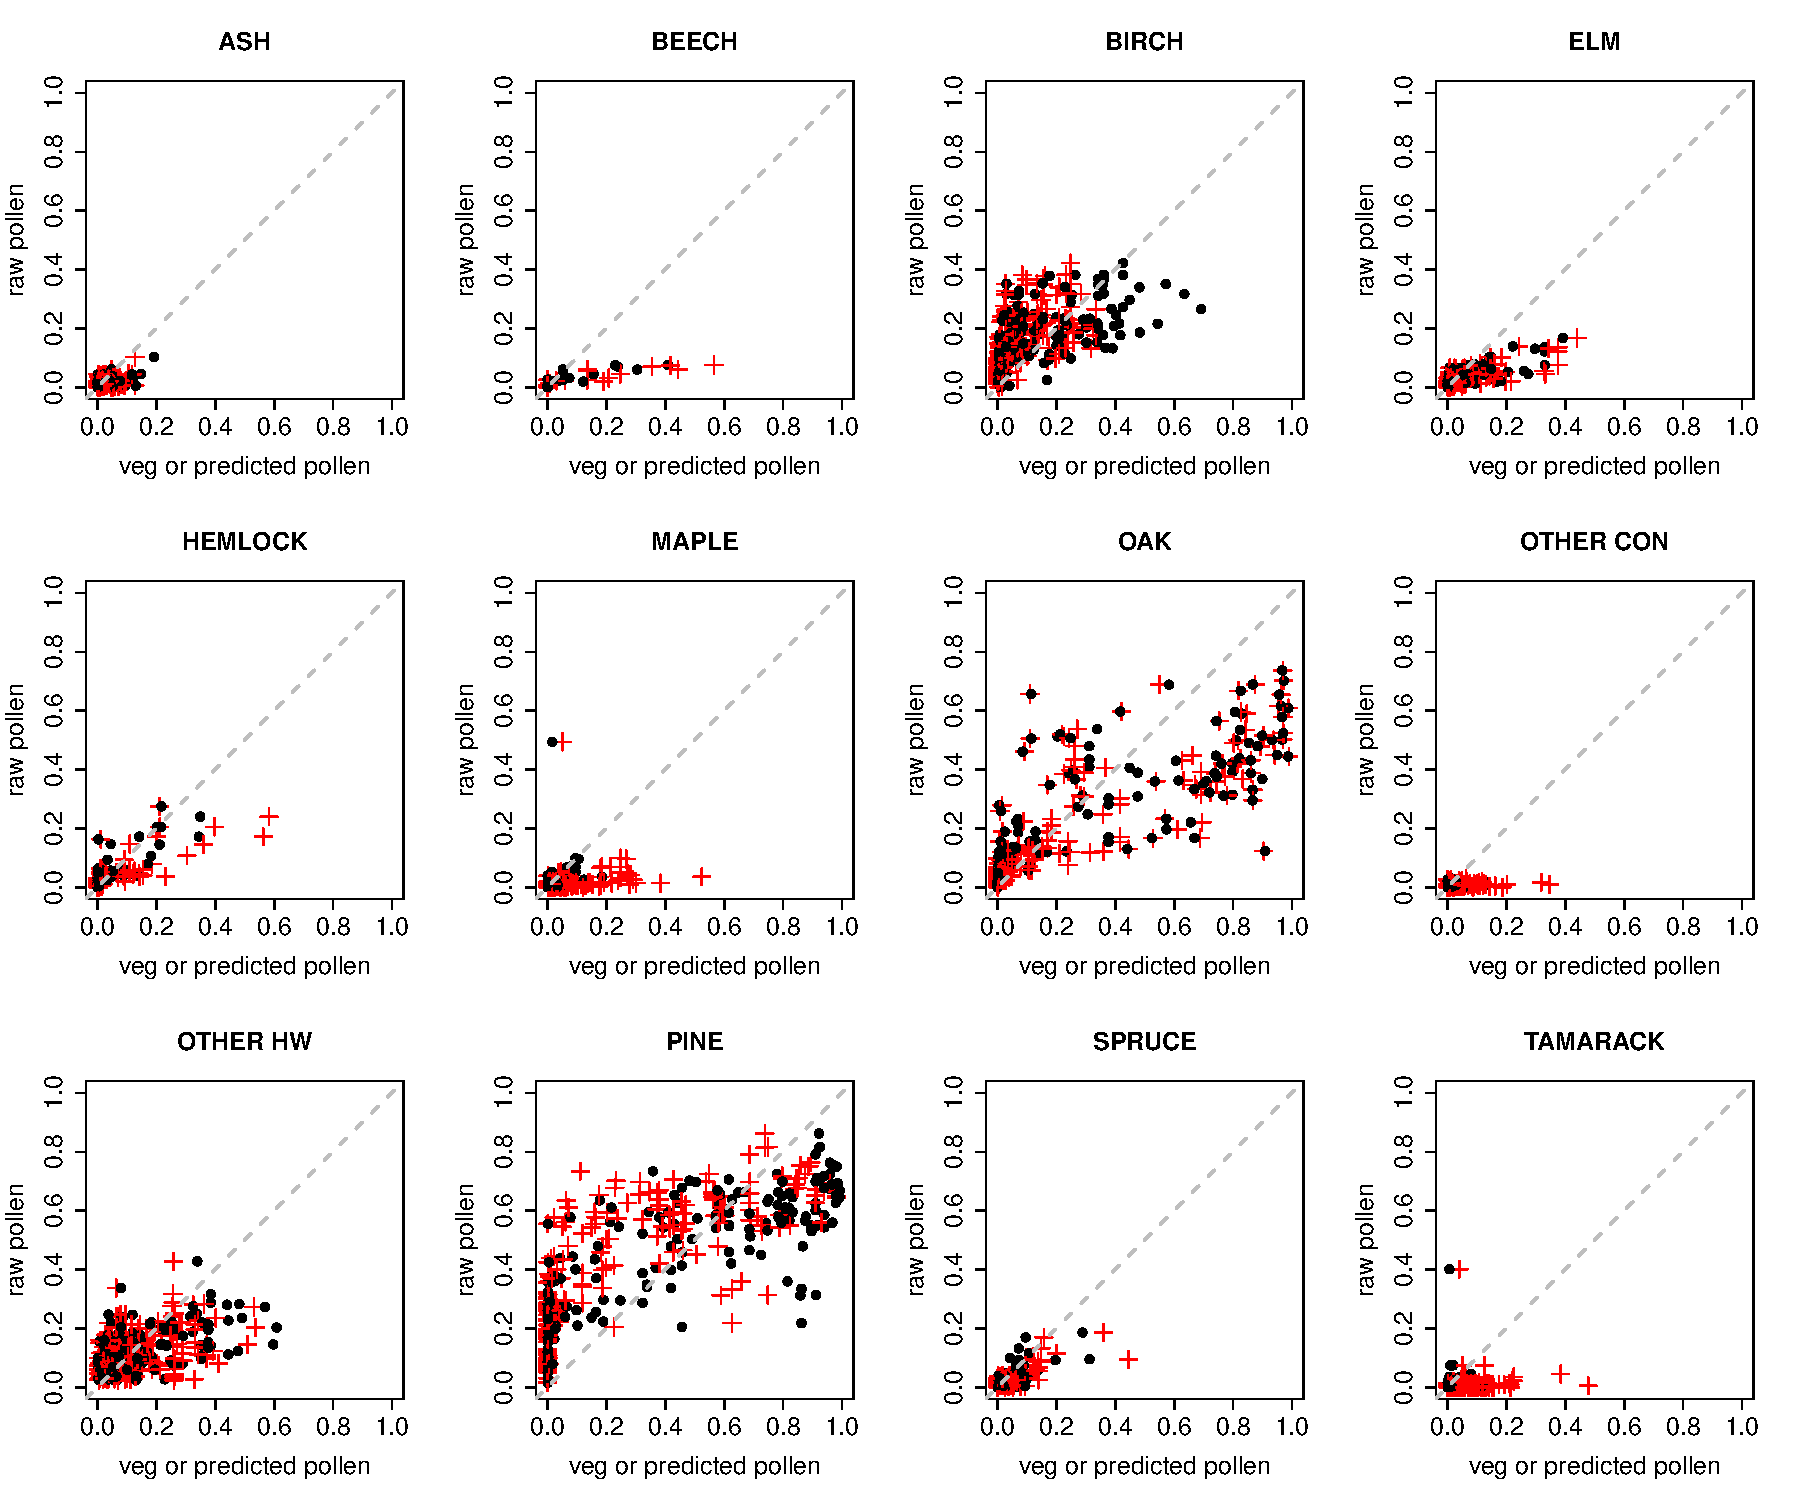
\includegraphics[width=7in]{figures/pollen_focal_scaled.pdf}
% \caption{}
% \label{fig:focal_scaled}
% \end{figure}

%PLS and pollen pie maps
\begin{figure}
\centering
\begin{tabular}{c}
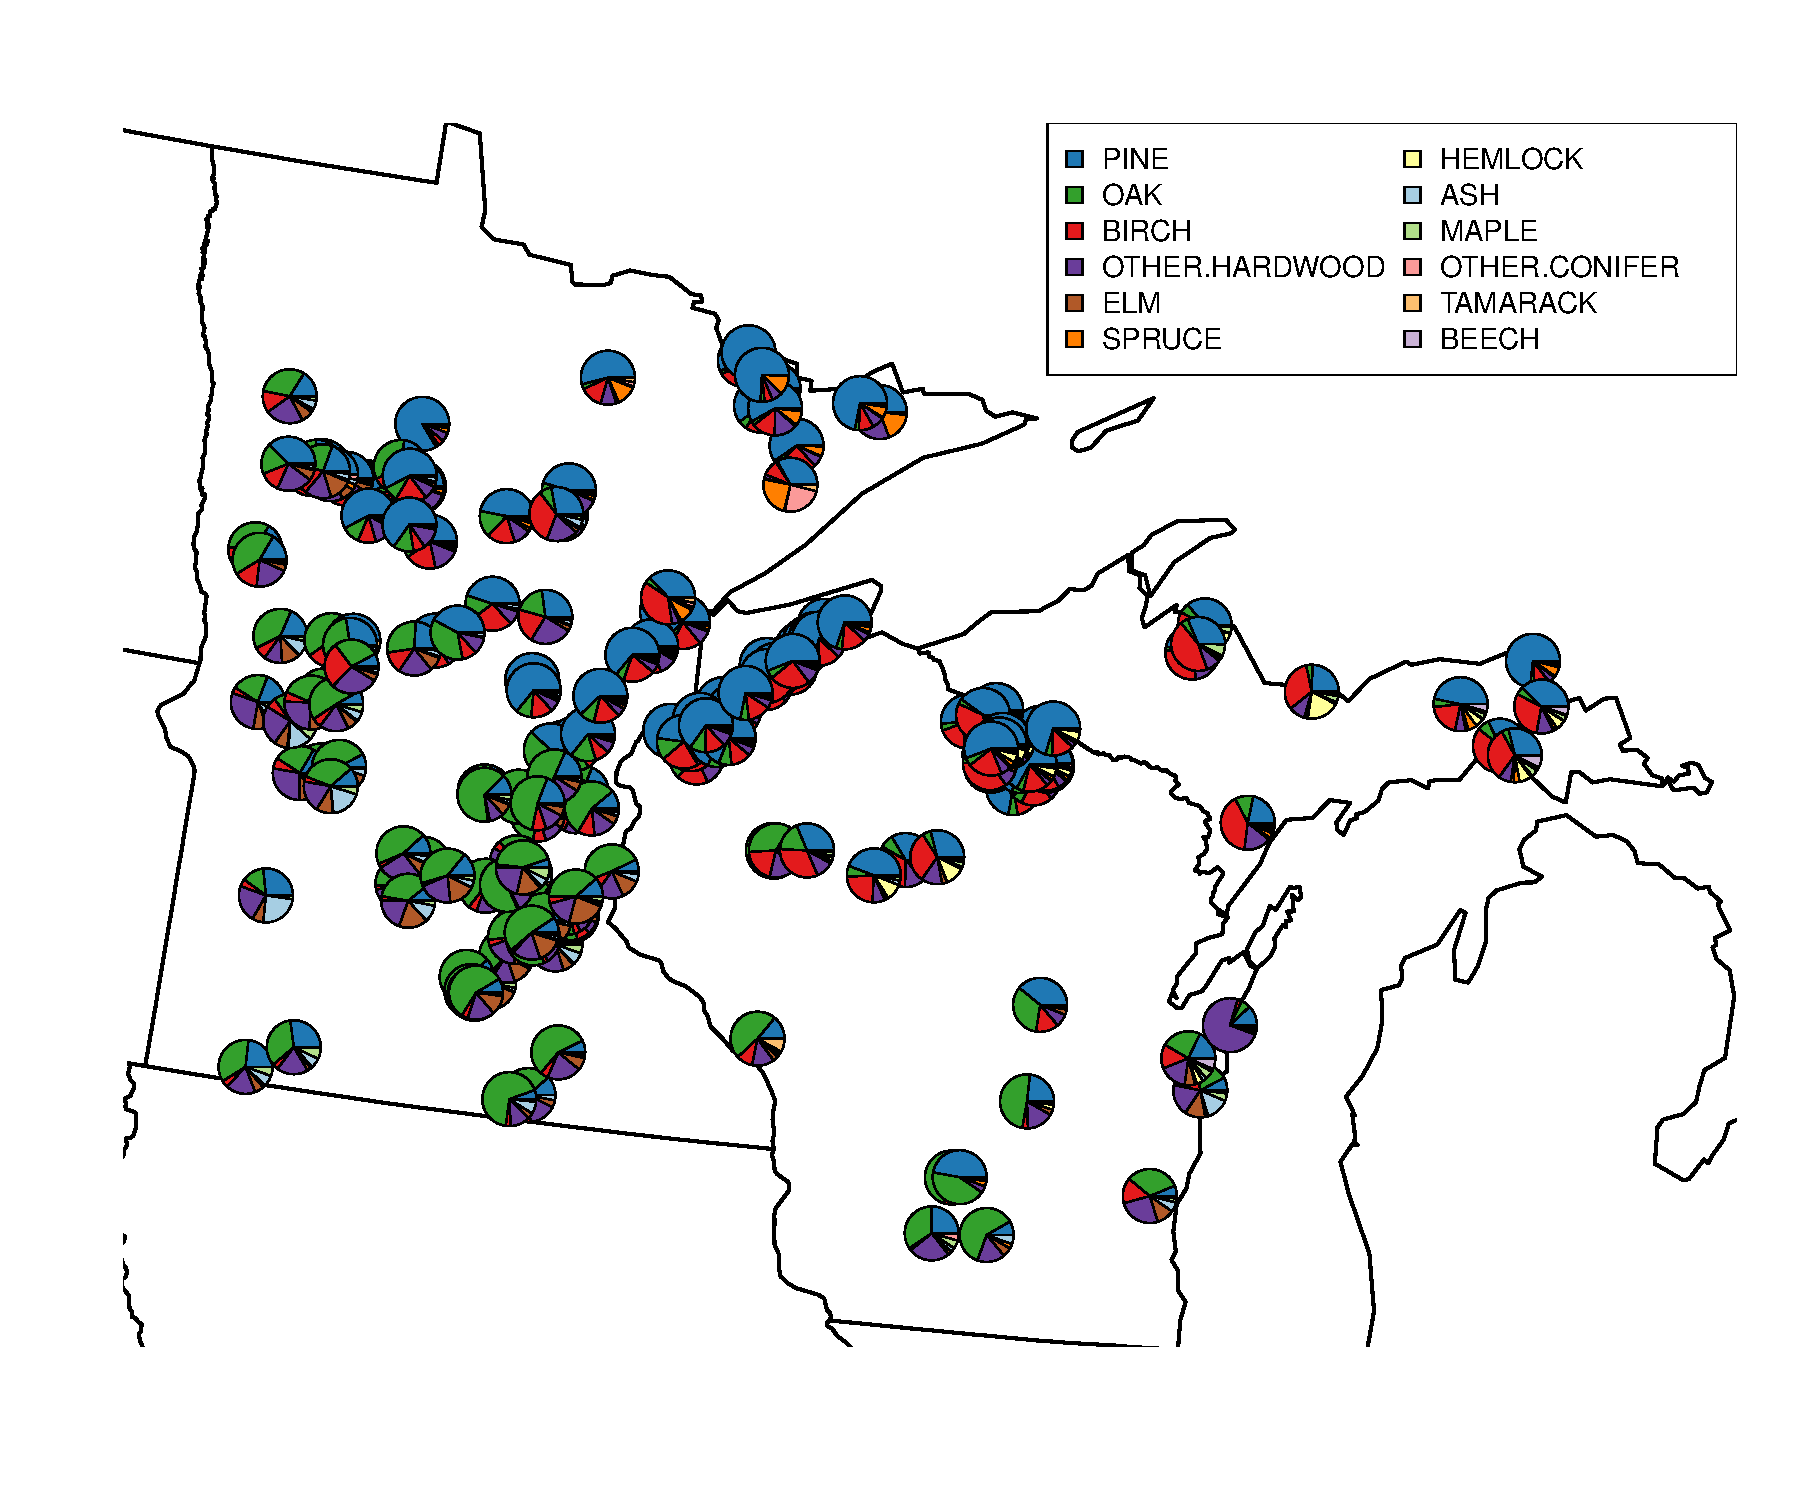
\includegraphics[width=5in]{figures/pie_plot_pollen_UMW_v01.pdf} \\
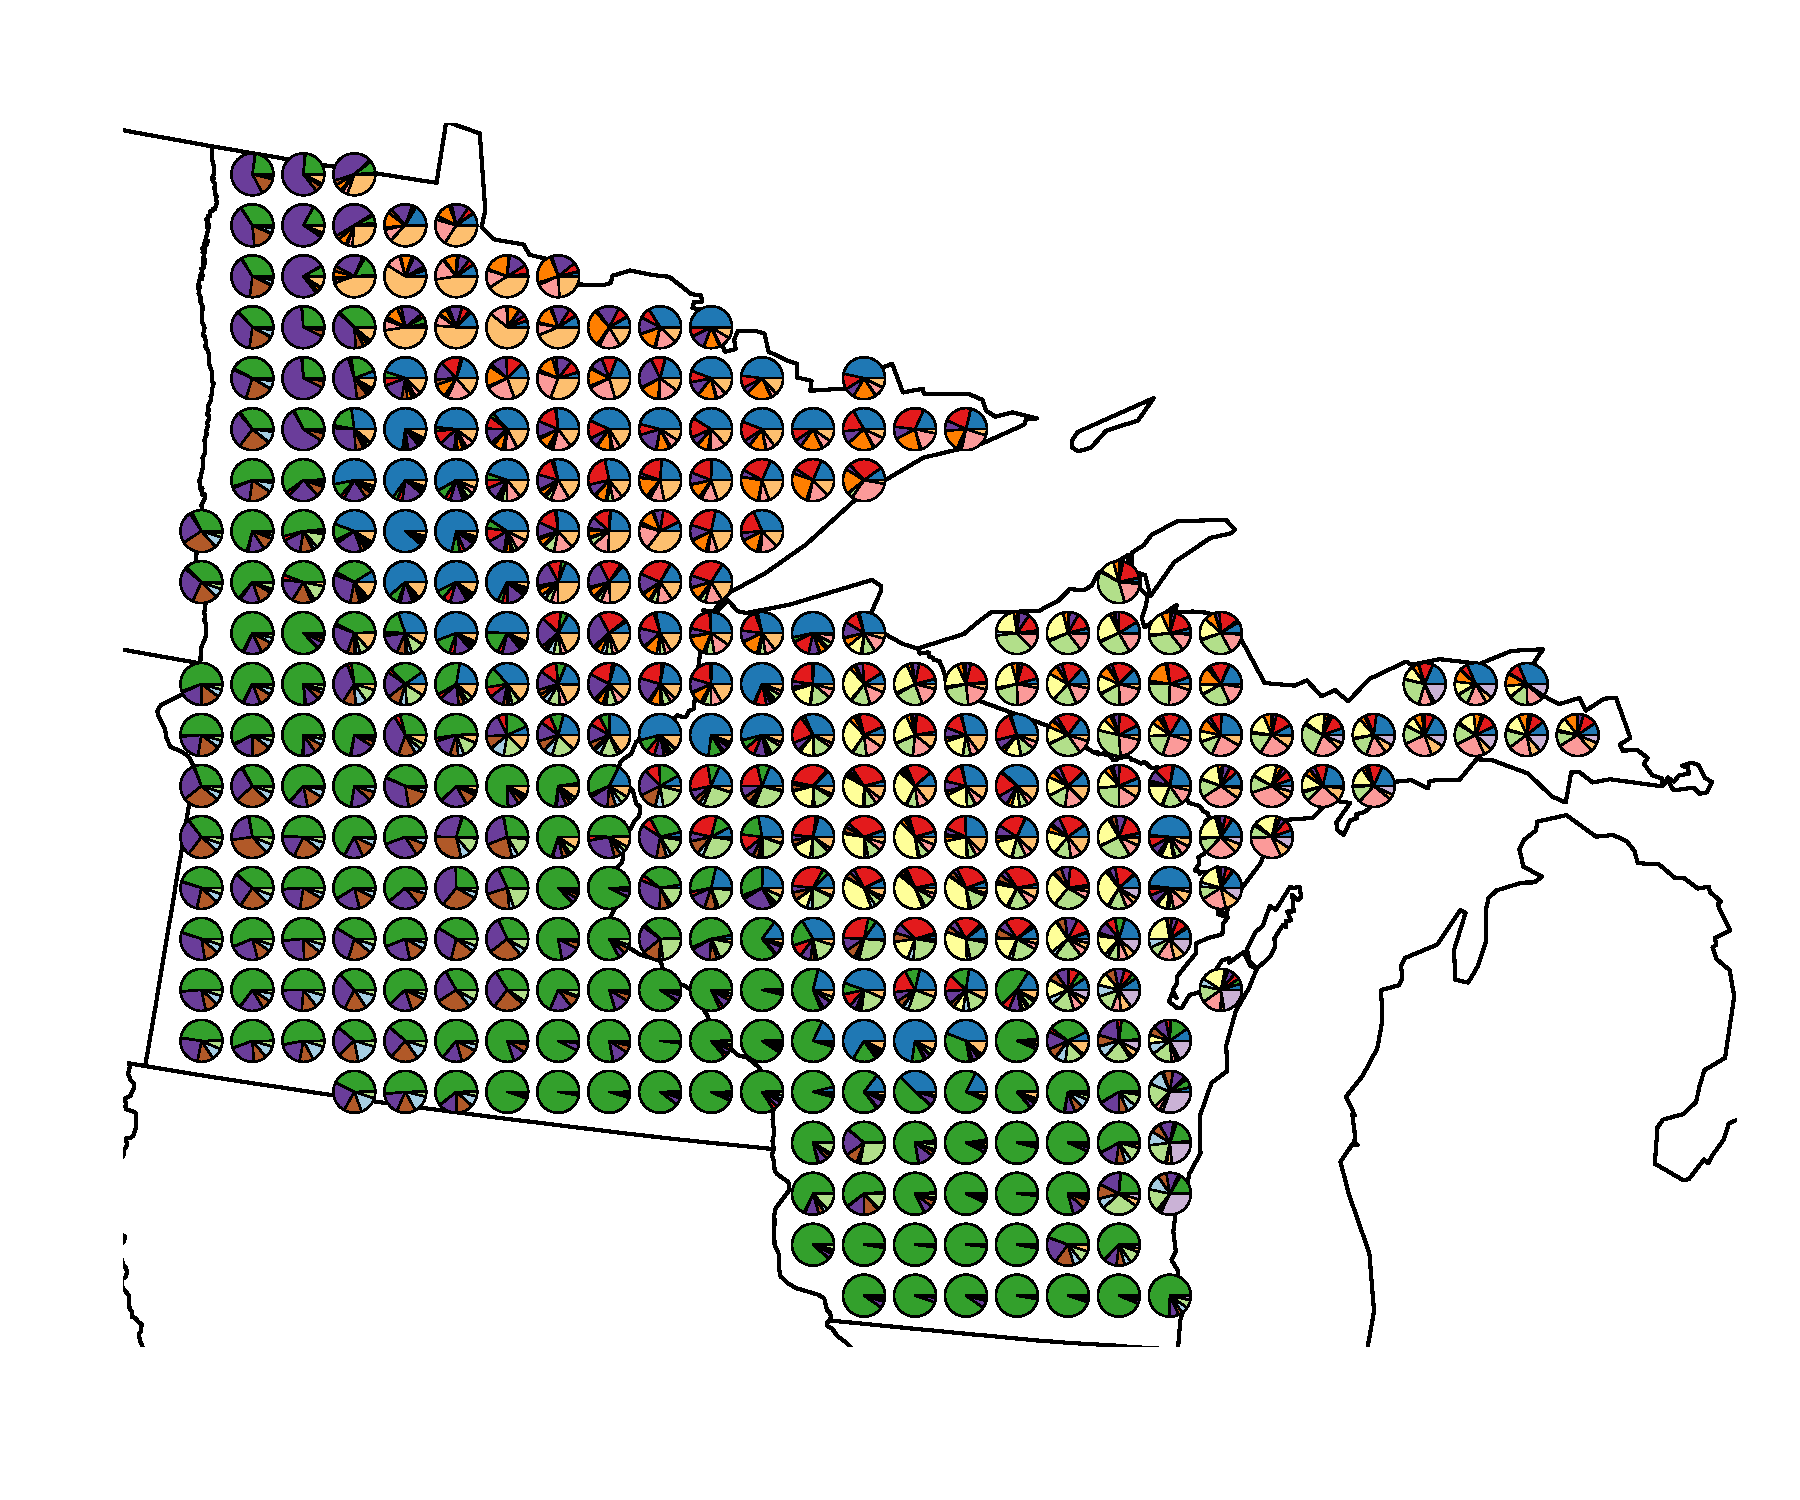
\includegraphics[width=5in]{figures/pie_plot_pls_UMW_v01.pdf}
\end{tabular}
\caption{Pie maps depicting the relative composition of pollen (top)
  and PLS vegetation (bottom) from the data. Note that the PLS data
  has been aggregated to a coarser resolution for illustrative
  purposes.}
\label{fig:pie}
\end{figure}

%veg and pollen heat maps: pine
\begin{figure}
\centering
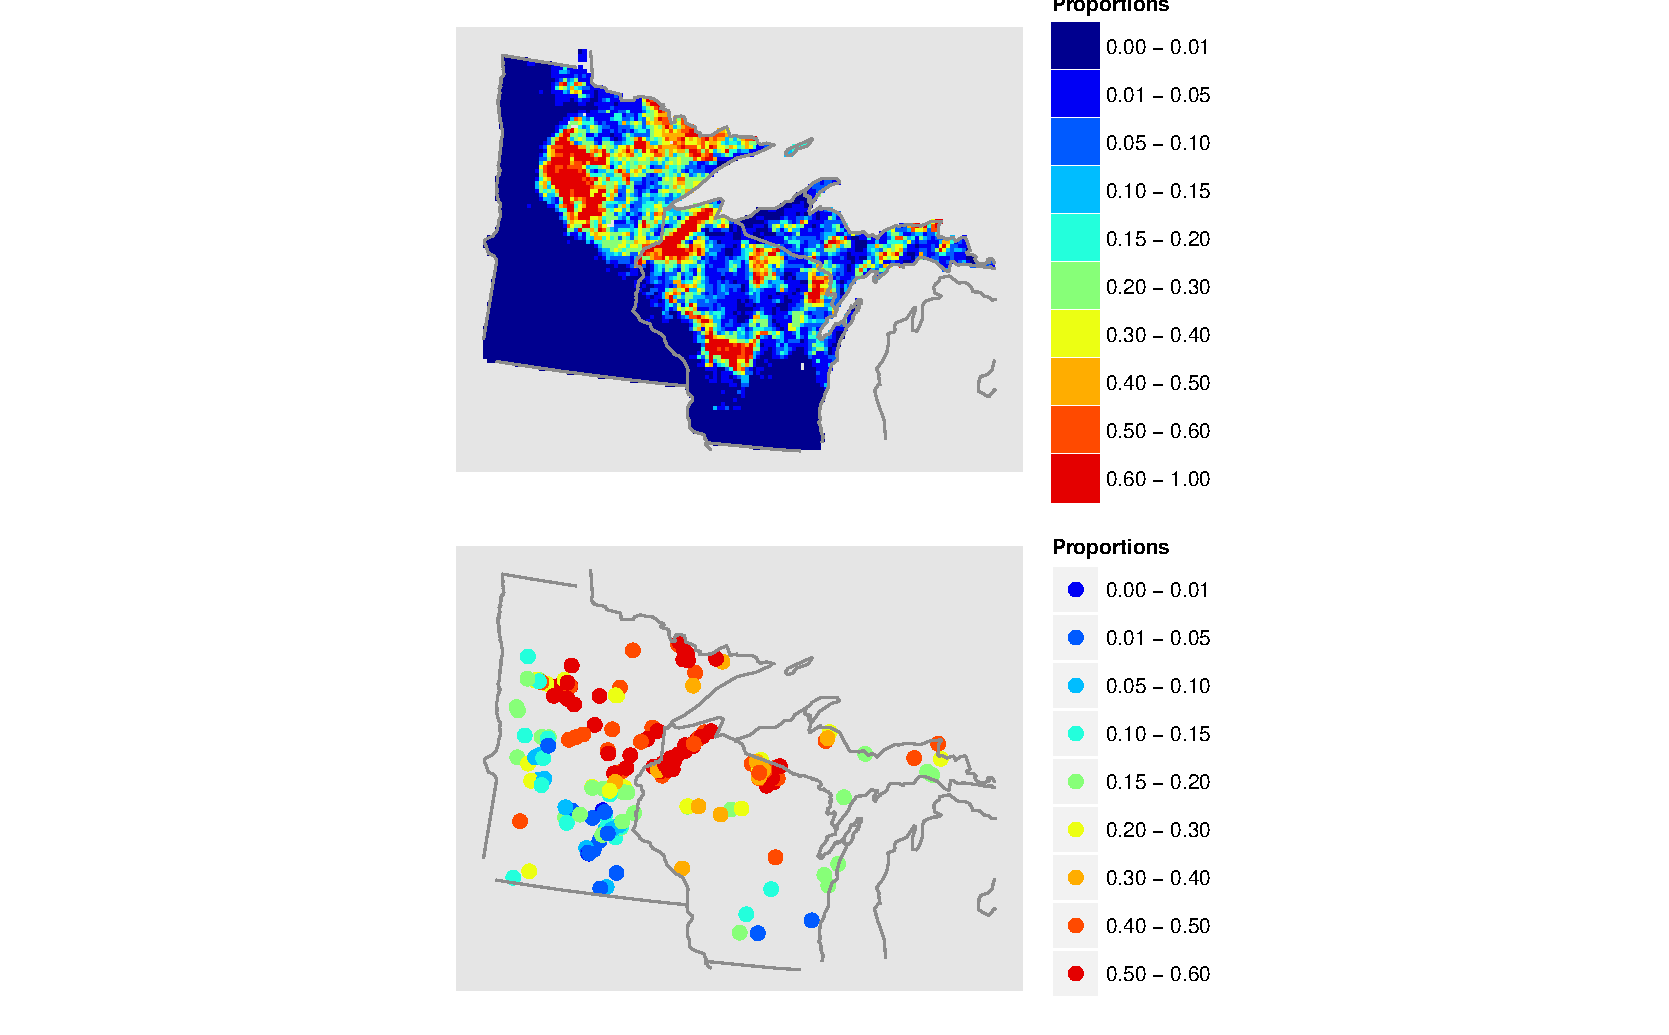
\includegraphics[width=7in]{figures/maps_compare_PINE.pdf}
\caption{Heat maps showing the range limits of Pine in the PLS composition data (top) and the sediment pollen (bottom).}
\label{fig:compare_maps_PINE}
\end{figure}

%veg and pollen heat maps: birch
\begin{figure}
\centering
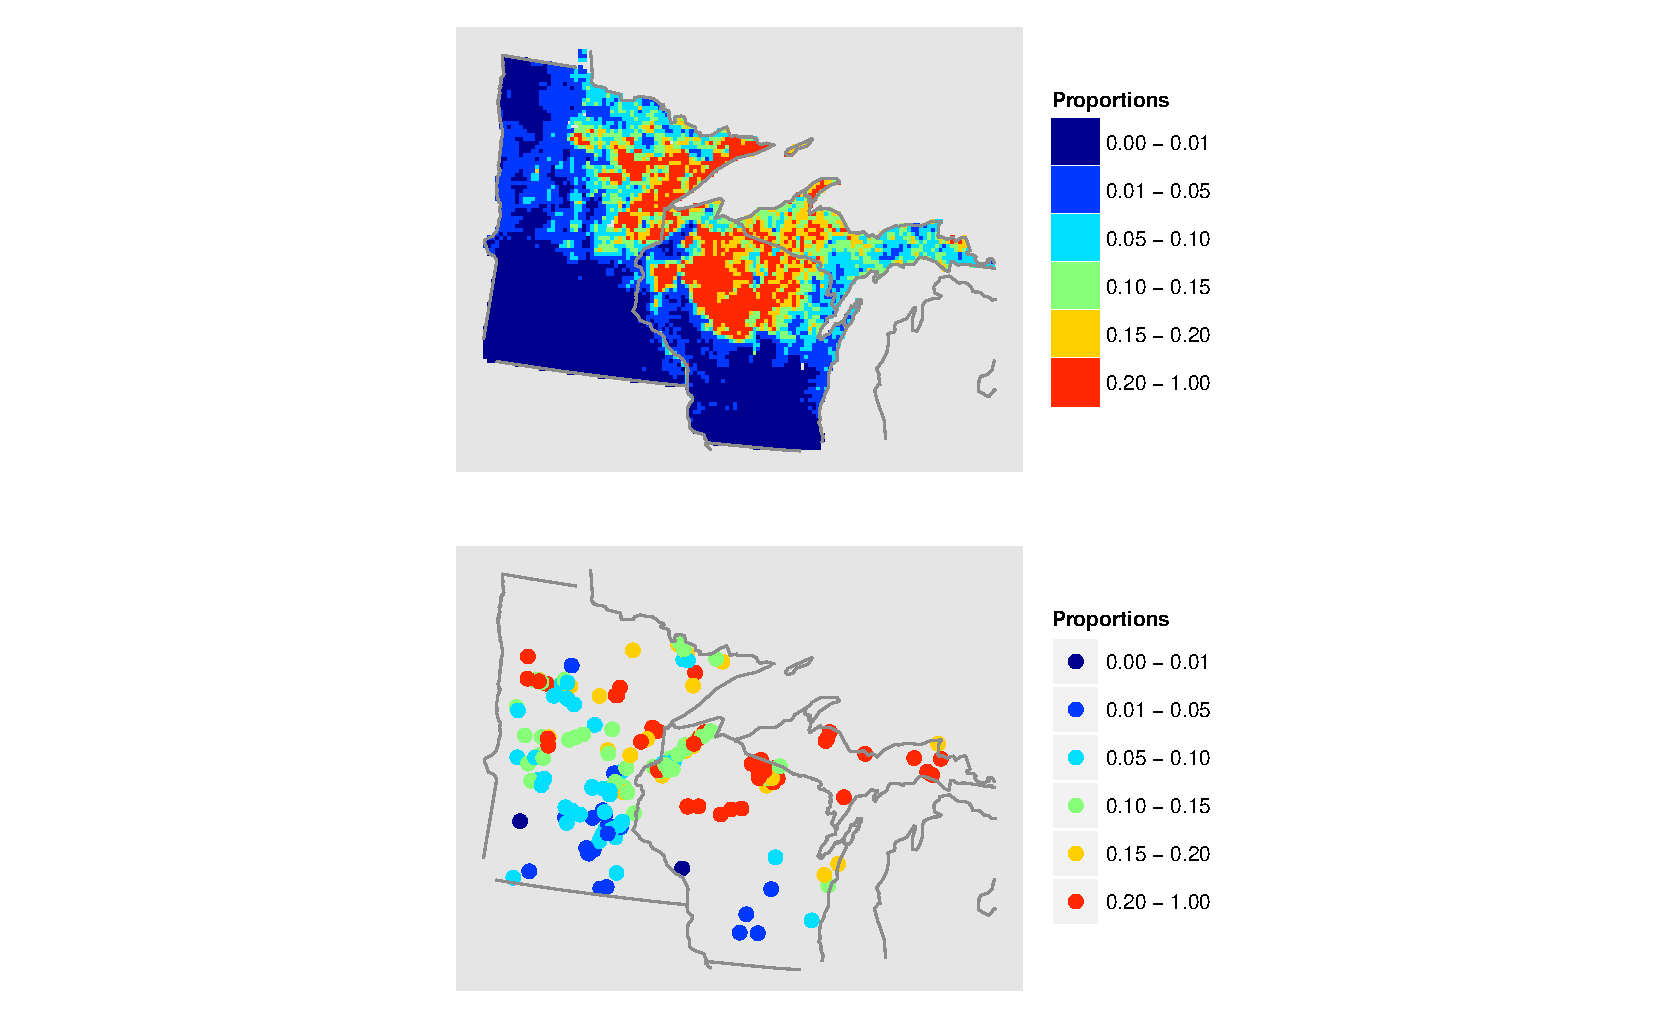
\includegraphics[width=7in]{figures/maps_compare_BIRCH.pdf}
\caption{Heat maps showing the range limits of Birch in the PLS composition data (top) and the sediment pollen (bottom)}
\label{fig:compare_maps_PINE}
\end{figure}

%pollen raw versus scaled focal
\begin{figure}
\centering
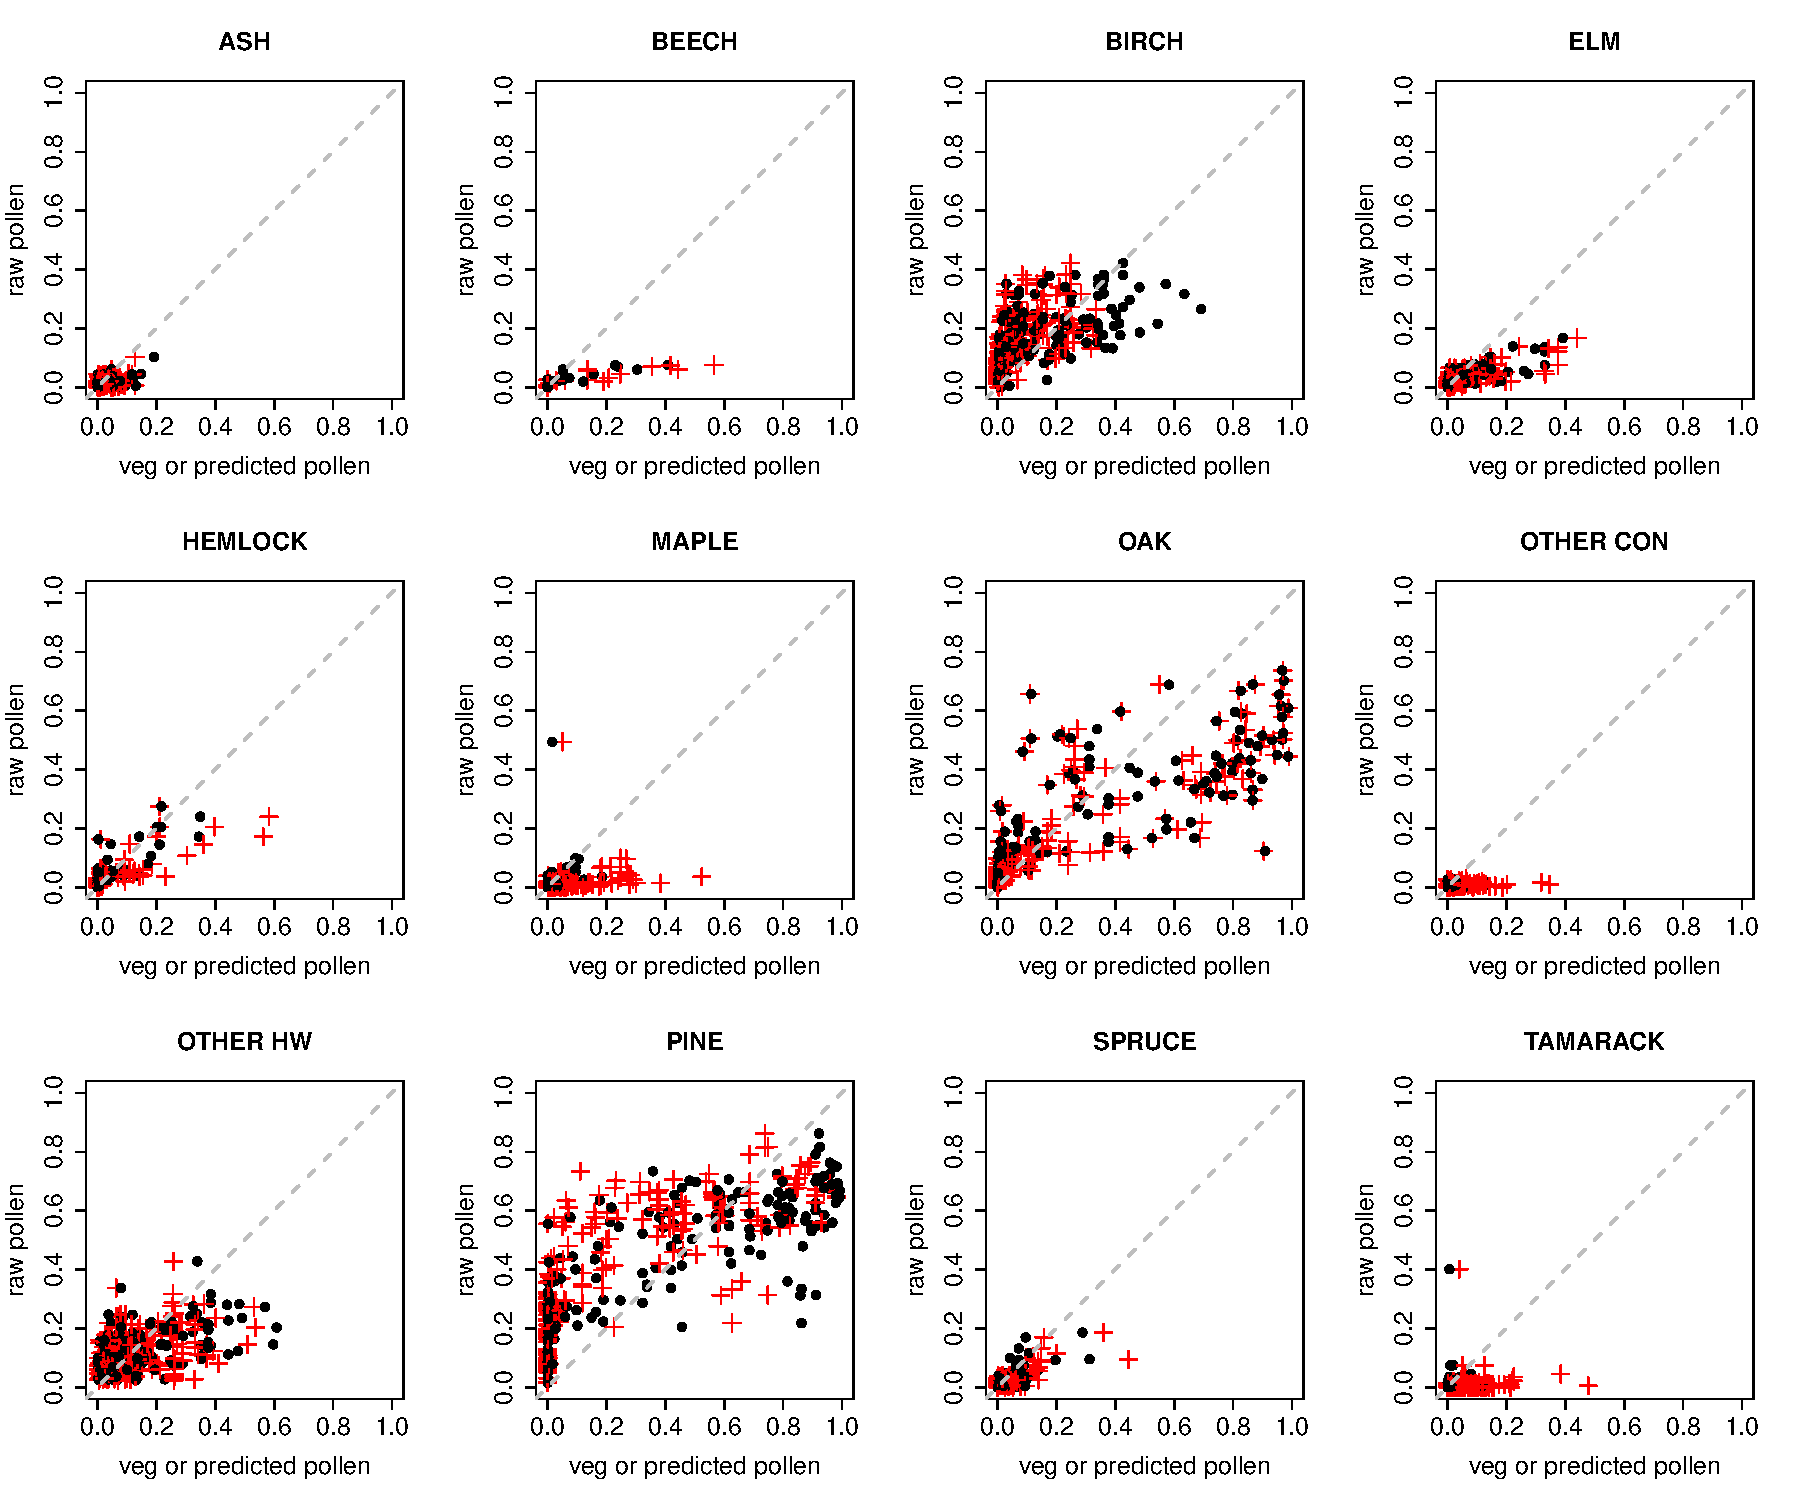
\includegraphics[width=7in]{figures/pollen_focal_scaled.pdf}
\caption{Pollen proportions plotted against local vegetation proportions (red crosses) or local vegetation proportion scaled by $\phi$ (black dots), by taxon.}
\label{fig:focal_scaled}
\end{figure}

%pollen raw versus predicted
\begin{figure}
\centering
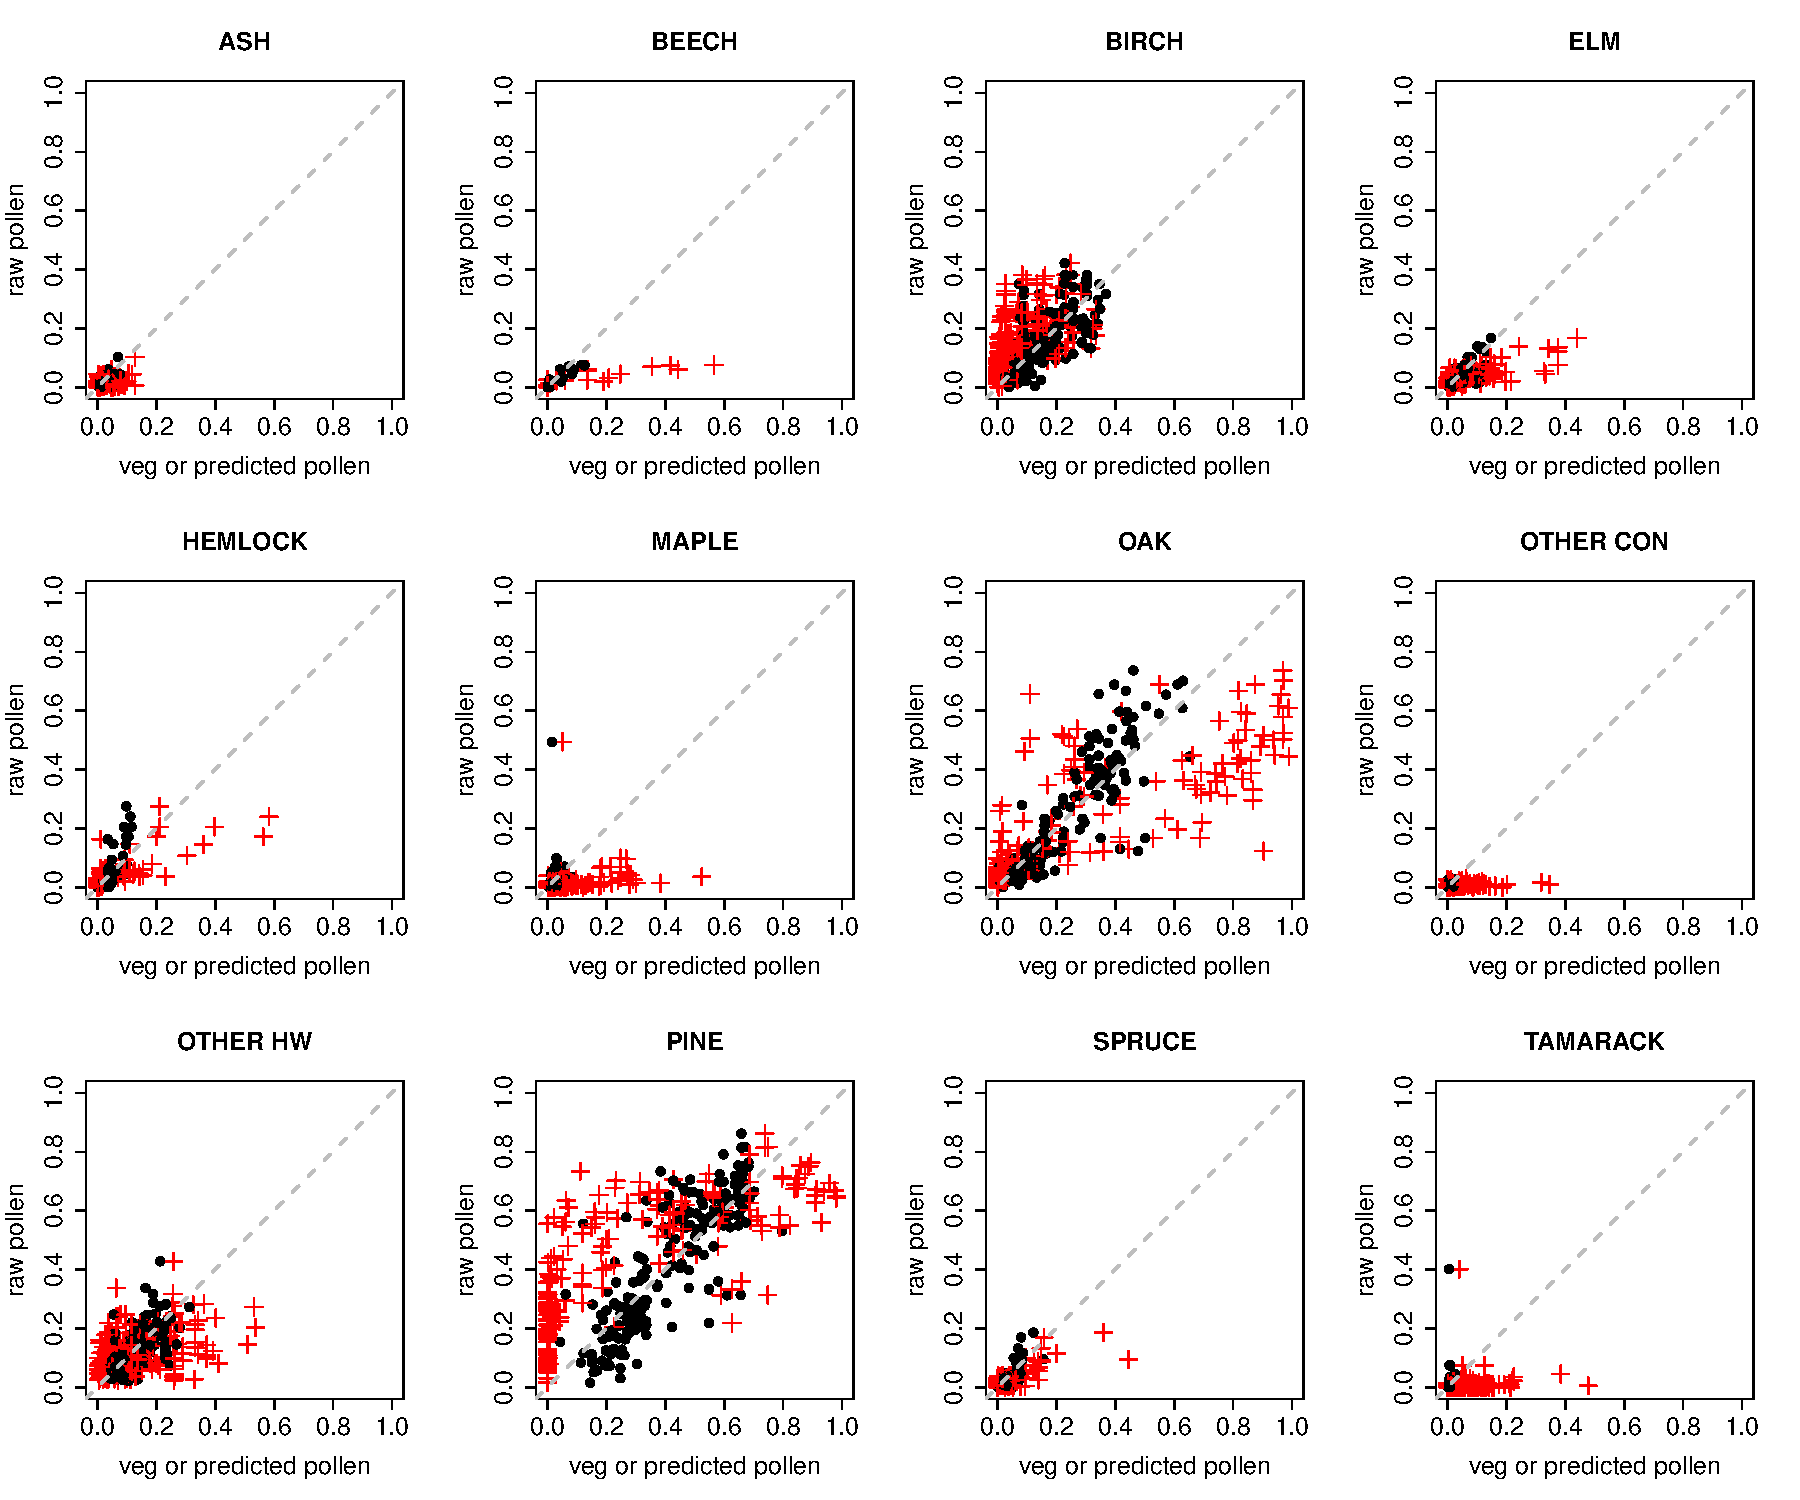
\includegraphics[width=7in]{figures/pollen_preds.pdf}
\caption{Pollen proportions plotted against local vegetation proportions (red crosses) or model-predicted pollen (black dots), by taxon.}
\label{fig:preds}
\end{figure}

%phi (differential production)
\begin{figure}
\centering
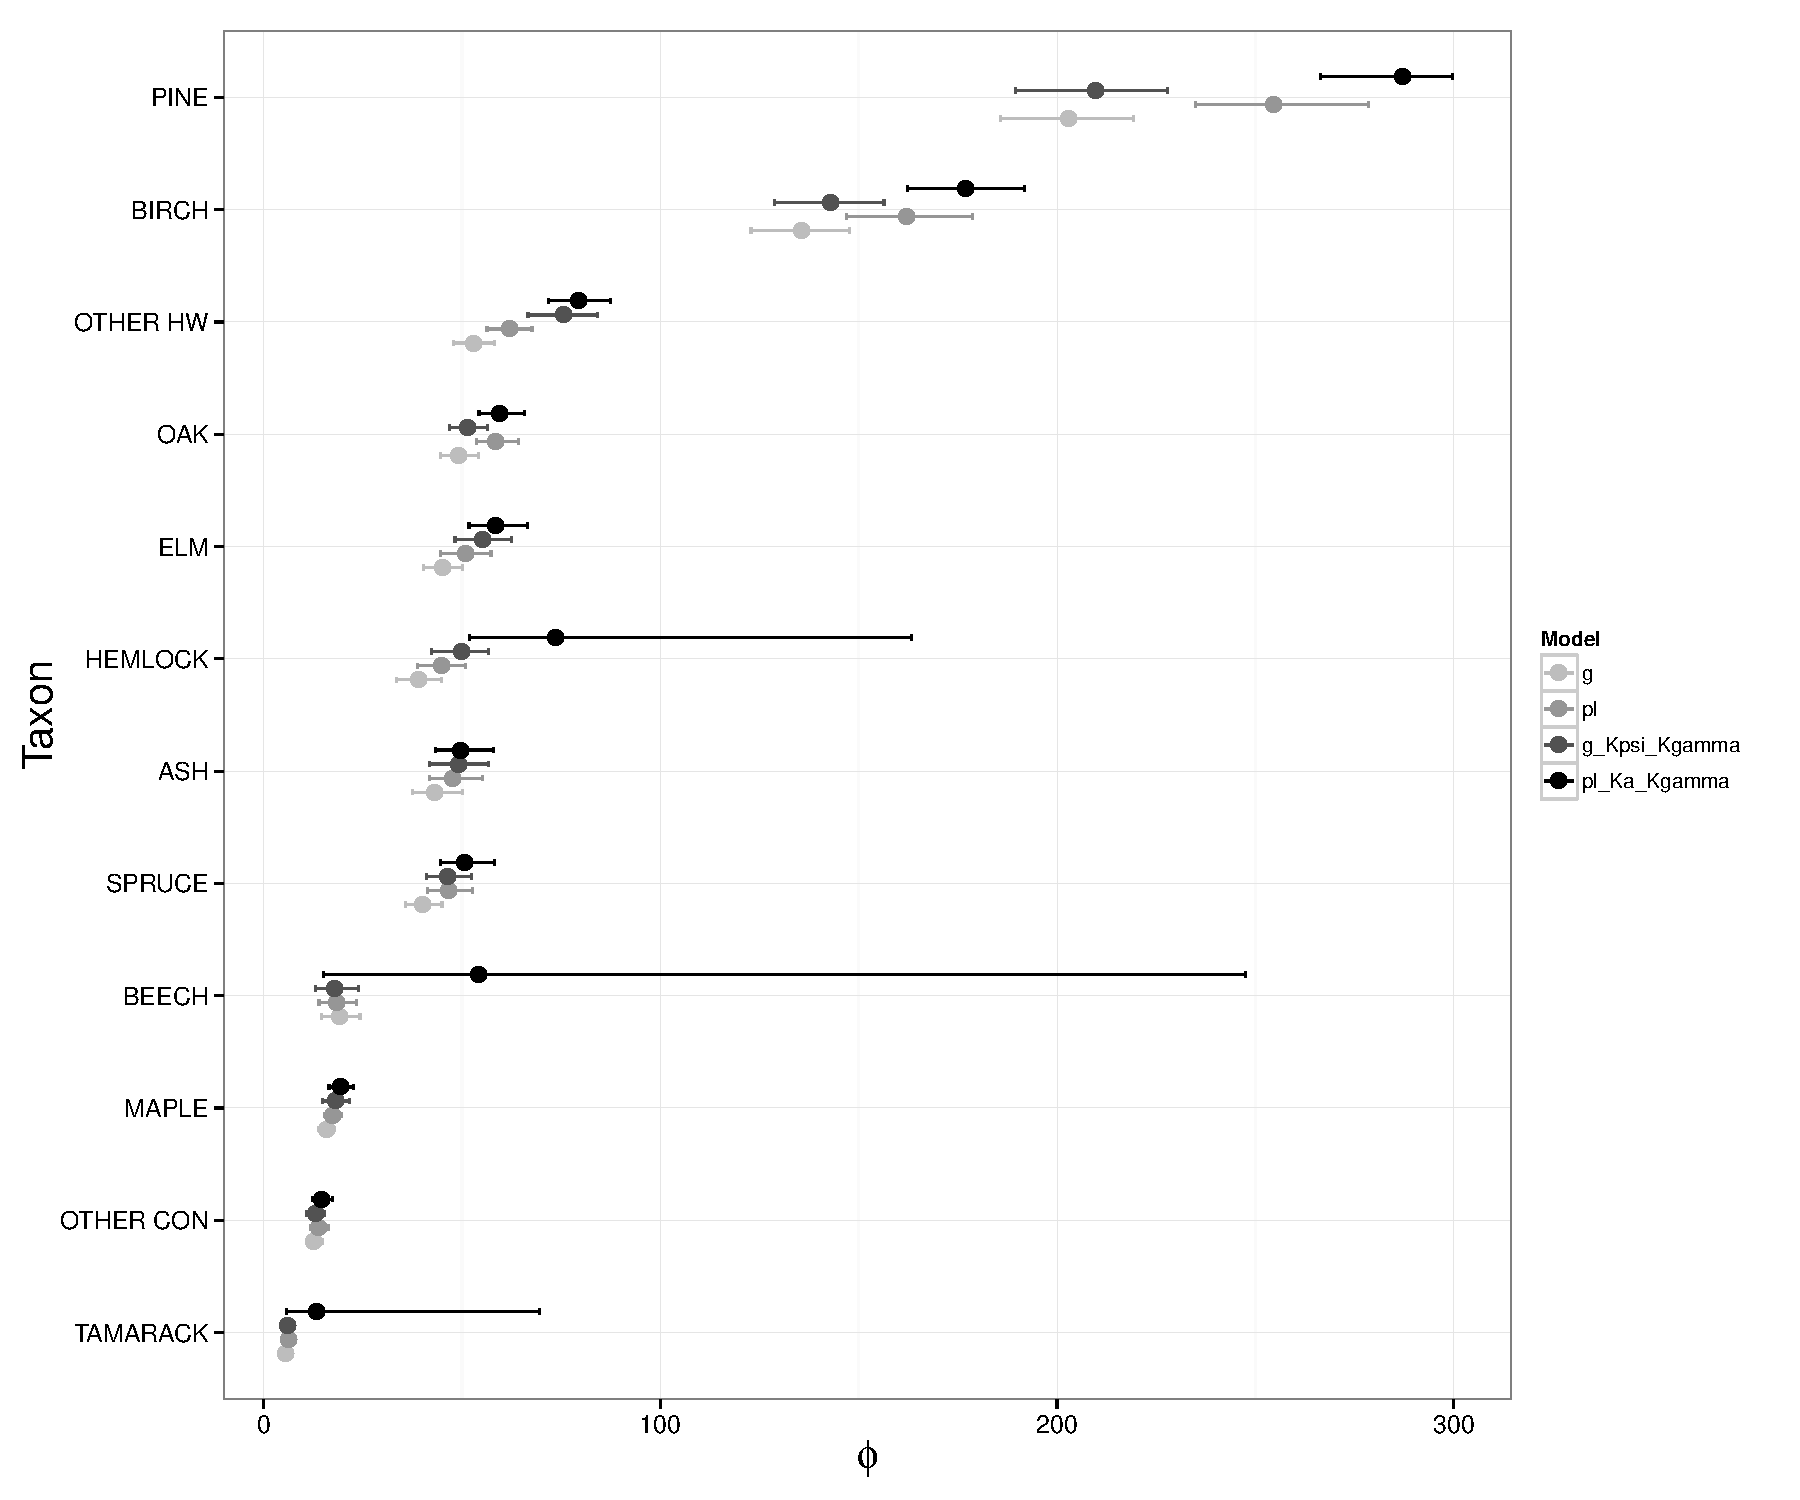
\includegraphics[width=7in]{figures/phi.pdf}
\caption{Mean values and 95\% credible intervals for the estimated values of the differential production parameter $\phi$.}
\label{fig:phi}
\end{figure}

%proportion pollen versus radius
\begin{figure}
\centering
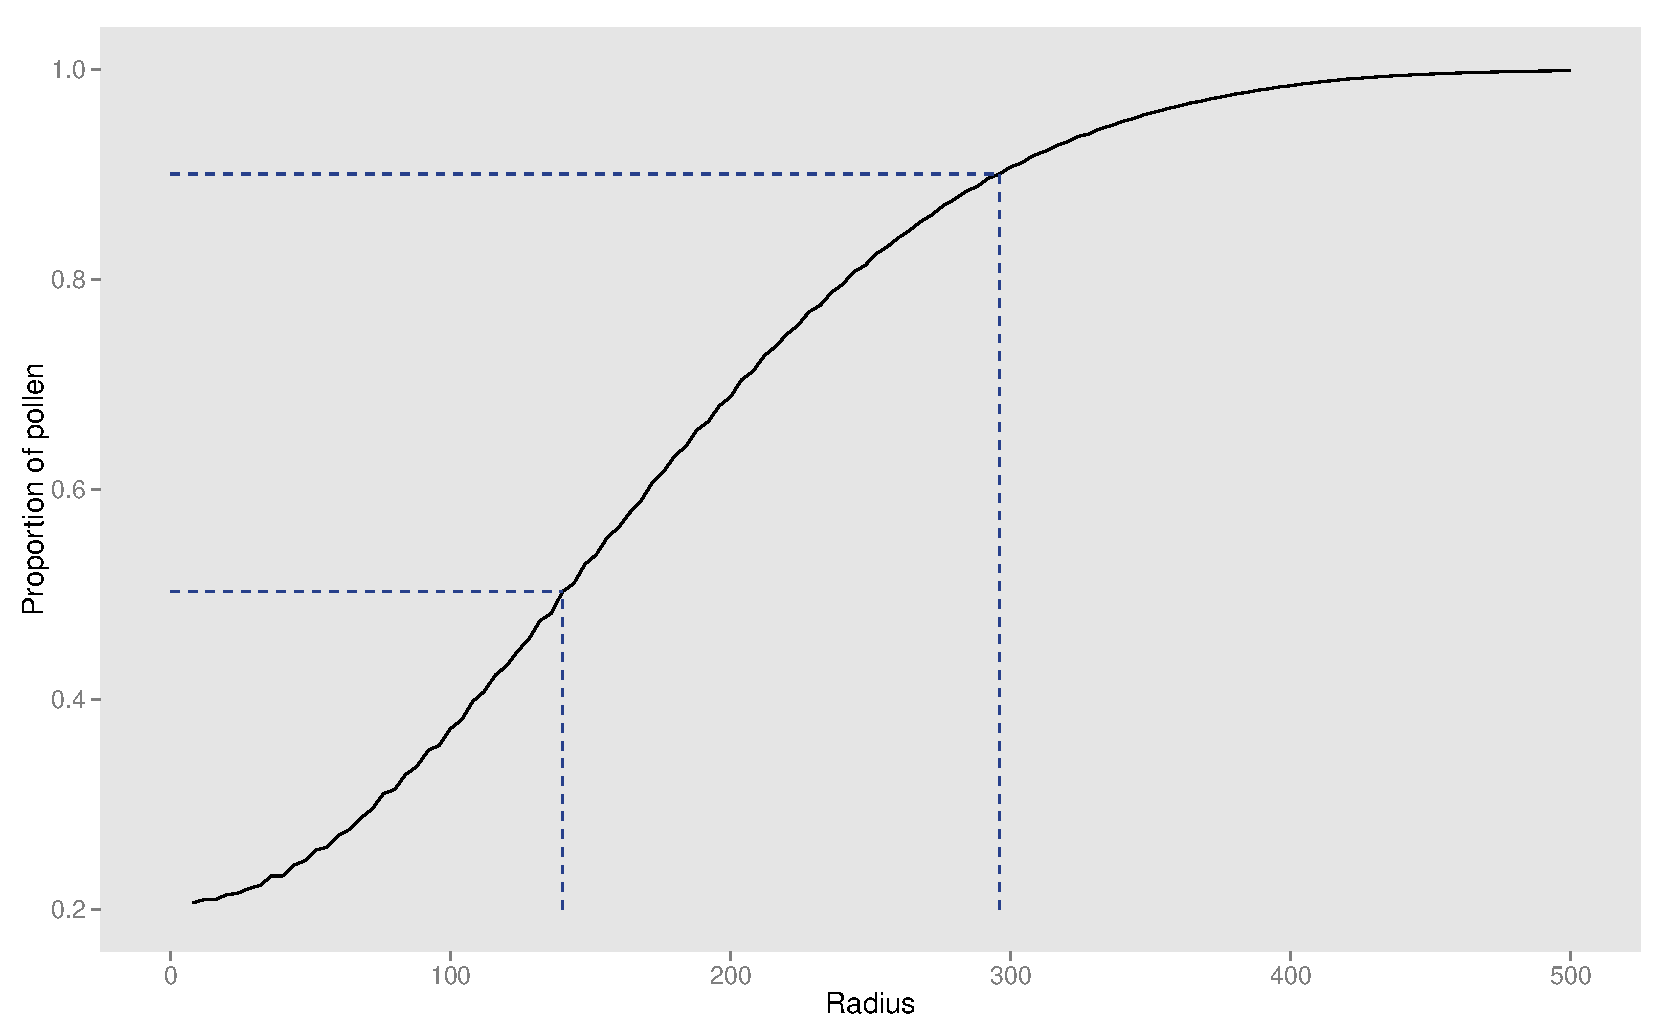
\includegraphics[width=7in]{figures/dispersal_vs_distance.pdf}
\caption{Here we consider pollen produced by a focal cell, and plot the proportion of deposited pollen as a function of the radius of a circle centered at the focal cell.}
\label{fig:dvd}
\end{figure}

%psi: vary psi case
\begin{figure}
\centering
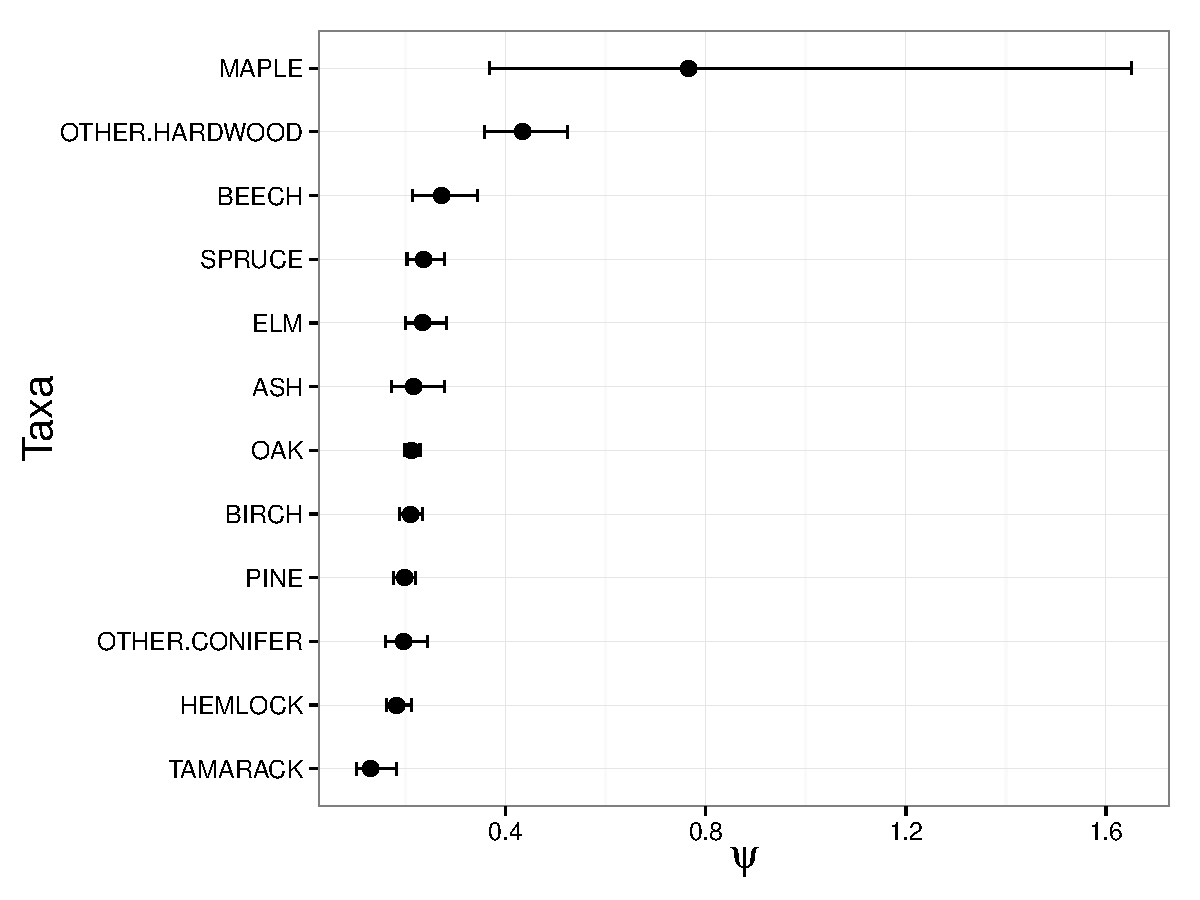
\includegraphics[width=7in]{figures/psi_vary_psi.pdf}
\caption{Mean values of 95\% credible intervals for the estimated values of the dispersal kernel spread $\psi$ for the case where we let $\psi$ vary by taxon.}
\label{fig:psi_vary_psi}
\end{figure}

%phi: vary phi case
\begin{figure}
\centering
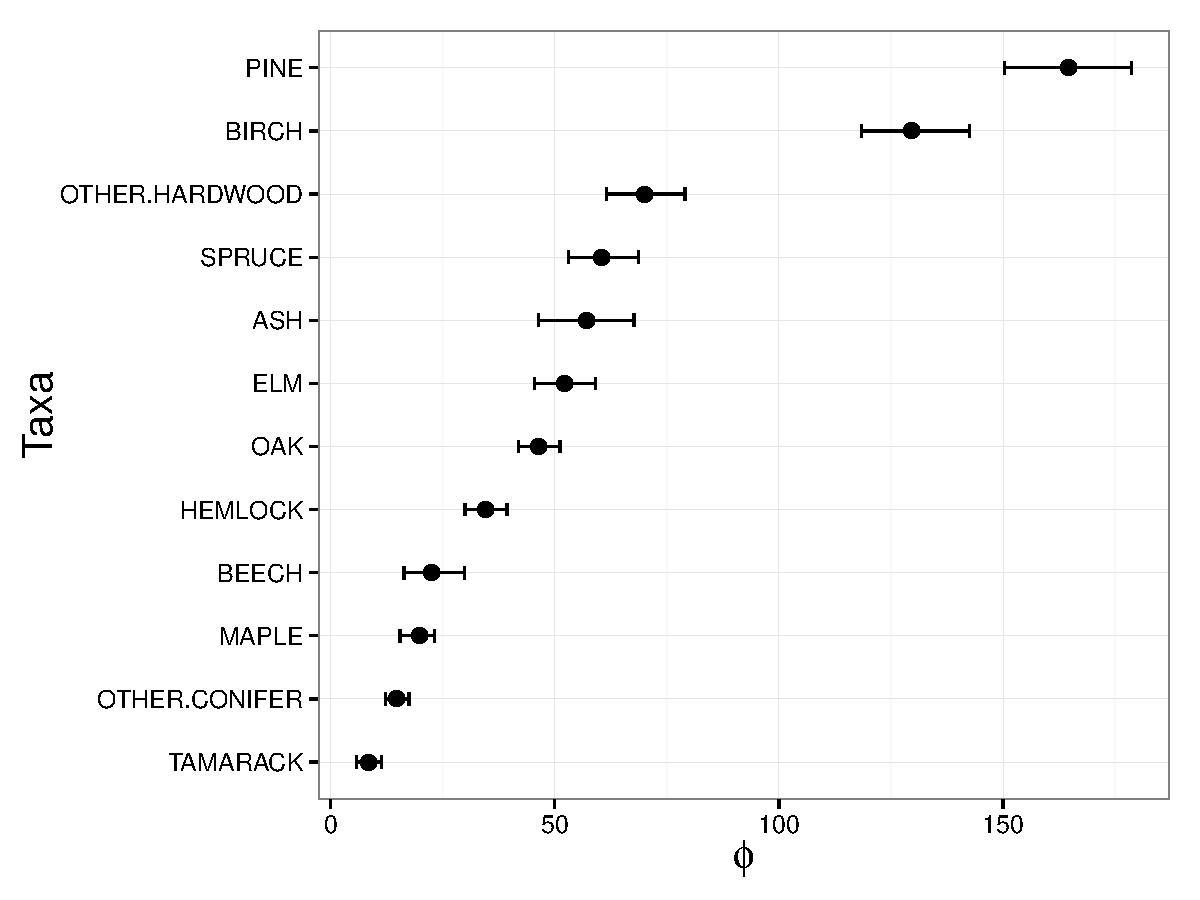
\includegraphics[width=7in]{figures/phi_vary_psi.pdf}
\caption{Mean values of 95\% credible intervals for the estimated values of the differential production parameter $\phi$ for the case where $\psi$ varied by taxon.}
\label{fig:phi_vary_psi}
\end{figure}

%potential pollen maps by taxon
\begin{figure}
\centering
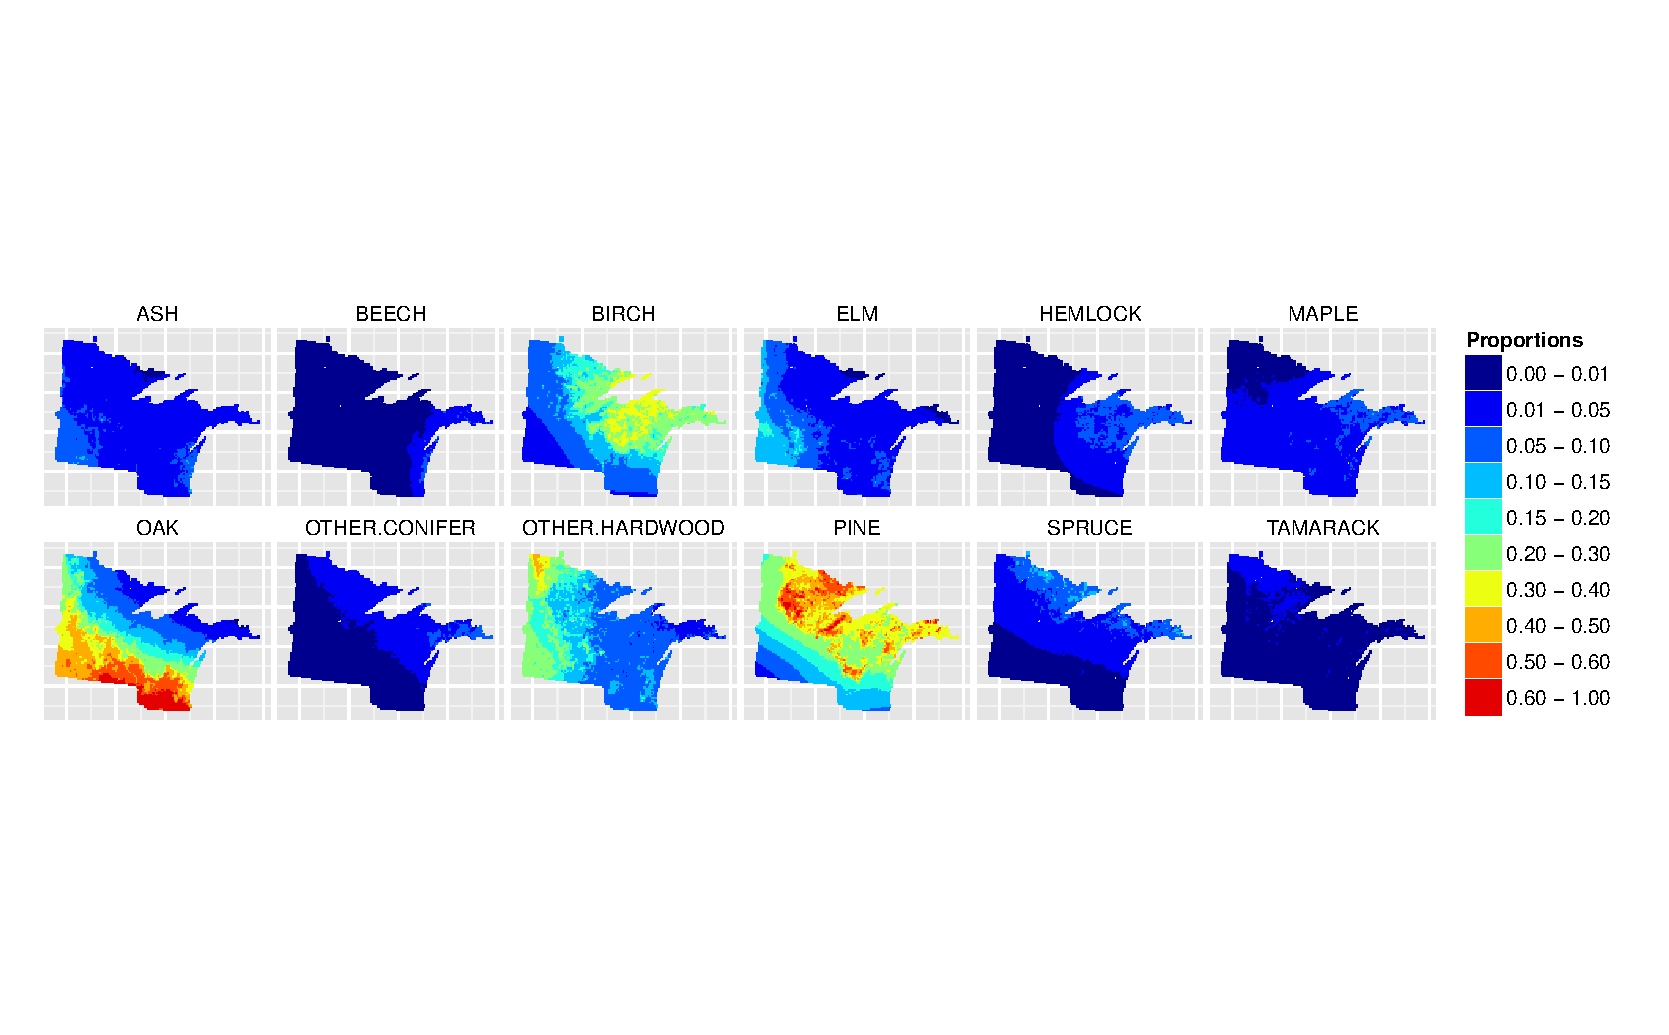
\includegraphics[width=7in]{figures/maps_pollen.pdf}
\caption{Heat maps of model-predicted pollen for each grid cell in the domain, by taxon.}
\label{fig:maps_pollen}
\end{figure}

%PLS data maps by taxon
\begin{figure}
\centering
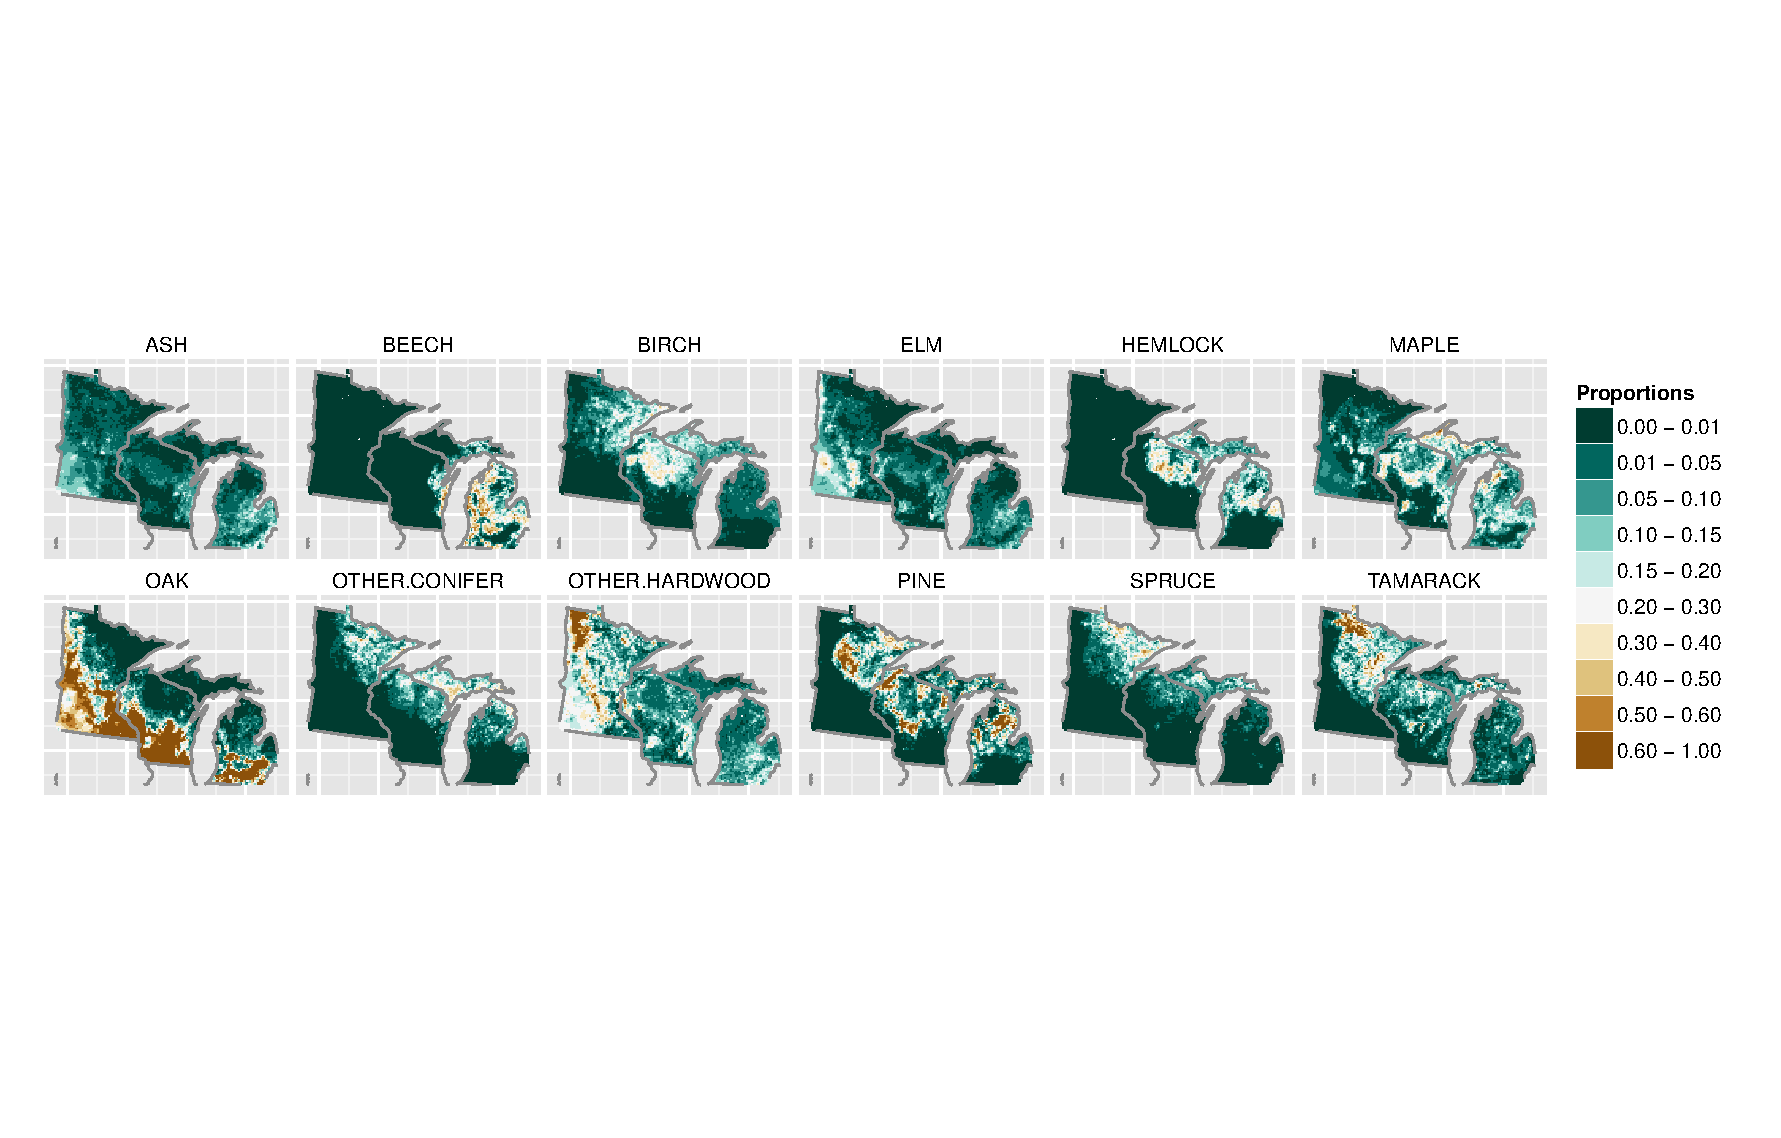
\includegraphics[width=7in]{figures/maps_veg.pdf}
\caption{Heat maps of the PLS data, by taxon.}
\label{fig:maps_pollen}
\end{figure}







\bibliography{calibration}

\end{document}
